\documentclass{beamer}
\usetheme{Boadilla}

\usepackage{eurosym}


\title{Next step}
\subtitle{TRITIUM}
\author{Marcos Martínez Roig}
\institute{University of Valencia}
\date{\today}

\begin{document}

\begin{frame}
\titlepage
\end{frame}

\begin{frame}
\frametitle{Outline}
\tableofcontents
\end{frame}

\section{PETSYS}
	\subsection{Bash code}
	\subsection{Id. Channels}
	\subsection{Scintillator Crystal}
	\subsection{Polishing effect with SiPM arrays}
	\subsection{Other posible studies}

\section{LARAM}
	\subsection{Polishing effect with PMTs}
	
\section{TRITIUM-IFIC 2}
	\subsection{Coincidence effect}
	\subsection{Effect to the lead}
	
\section{TRITIUM-IFIC 3}

\section{Future studies}


\begin{frame}
\frametitle{PETSYS. Bash code}
\begin{itemize}
\item{} I have modified Configure-calibration.sh file

\begin{figure}[hbtp]
\centering
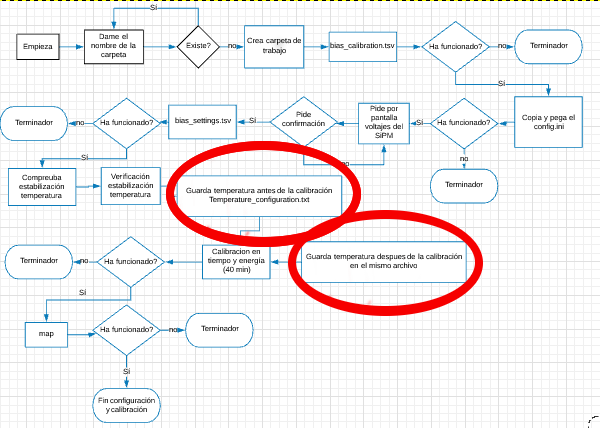
\includegraphics[scale=0.4]{PETSYS/Bash_code/Modification_Configure.png}
\caption{I save the temperature before and after calibration}
\end{figure}


\end{itemize}

\end{frame}

\begin{frame}
\frametitle{PETSYS. Bash code}
\begin{itemize}
\item{} I have modified Acquire.sh file

\begin{figure}[hbtp]
\centering
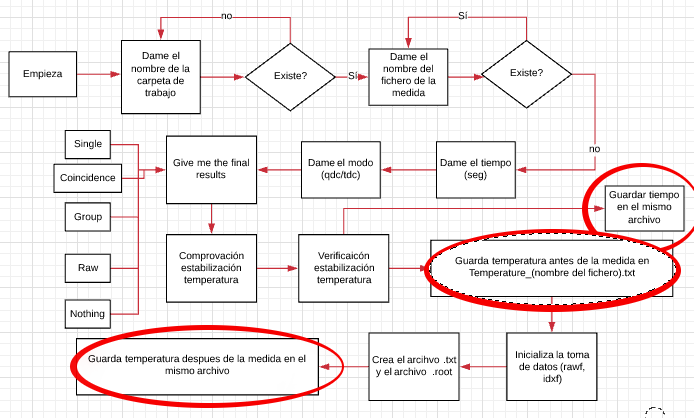
\includegraphics[scale=0.45]{PETSYS/Bash_code/Modification_Acquire.png}
\caption{I save the temperature before and after measurement}
\end{figure}


\end{itemize}

\end{frame}

\begin{frame}
\frametitle{PETSYS. Id. Channel}
\begin{itemize}
\item{} PETSYS system.

\begin{columns}
\column{0.5\textwidth}

\begin{figure}[hbtp]
\centering
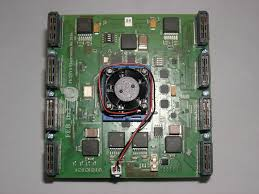
\includegraphics[scale=0.5]{PETSYS/Id_channel/8_ports.jpeg}
\caption{PETSYS system has 8 ports}
\end{figure}

\column{0.5\textwidth}

Channel clasification:
\begin{itemize}
\item{} 0-127 (0-63 and 64- 127)
\item{} 128-255 (128-191 and 192-255)
\item{} 256-383 (256-319 and 320-383)
\item{} 384-511 (384-447 and 448-511)
\item{} 512-639 (512-575 and 576-639)
\item{} 640-767 (640-703 and 704-767)
\item{} 768-895 (768-831 and 832-895)
\item{} 895-1023 (895-959 and 960-1023)
\end{itemize}

\end{columns}

\end{itemize}

\end{frame}

\begin{frame}
\frametitle{PETSYS. Id. Channel}
\begin{itemize}
\item{} PETSYS system.

\begin{columns}
\column{0.5\textwidth}

\begin{figure}[hbtp]
\centering
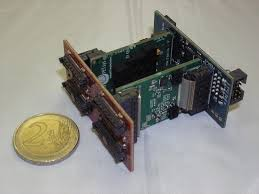
\includegraphics[scale=0.5]{PETSYS/Id_channel/TOFPET.jpeg}
\caption{Each TOFPET has 128 channels (32x4)}
\end{figure}

\column{0.5\textwidth}

\begin{itemize}
\item{} 2 symmetric parts each one with 64 channels (0-127):
\begin{itemize}
\item{} 0-63
\item{} 64-127
\end{itemize}
\item{} We connect a SiPM array in each part.
\begin{itemize}
\item{} If we use 8x8 SiPM arrays each channel correspont to a different SiPM (64 SiPMs)
\item{} If we use 4x4 SiPM arrays we have to see how our SiPM give us this information (16 SiPMs)$\longrightarrow$ Hammamatsu Photonics use four channels in each SiPM (16x4=64)
\item{} Question!!
\end{itemize}

\end{itemize}

\end{columns}

\end{itemize}

\end{frame}








\begin{frame}
\frametitle{PETSYS. Id. Channel}
\begin{itemize}
\item{} I have designed and built a 3D piece.

\begin{columns}
\column{0.5\textwidth}

\begin{figure}[hbtp]
\centering
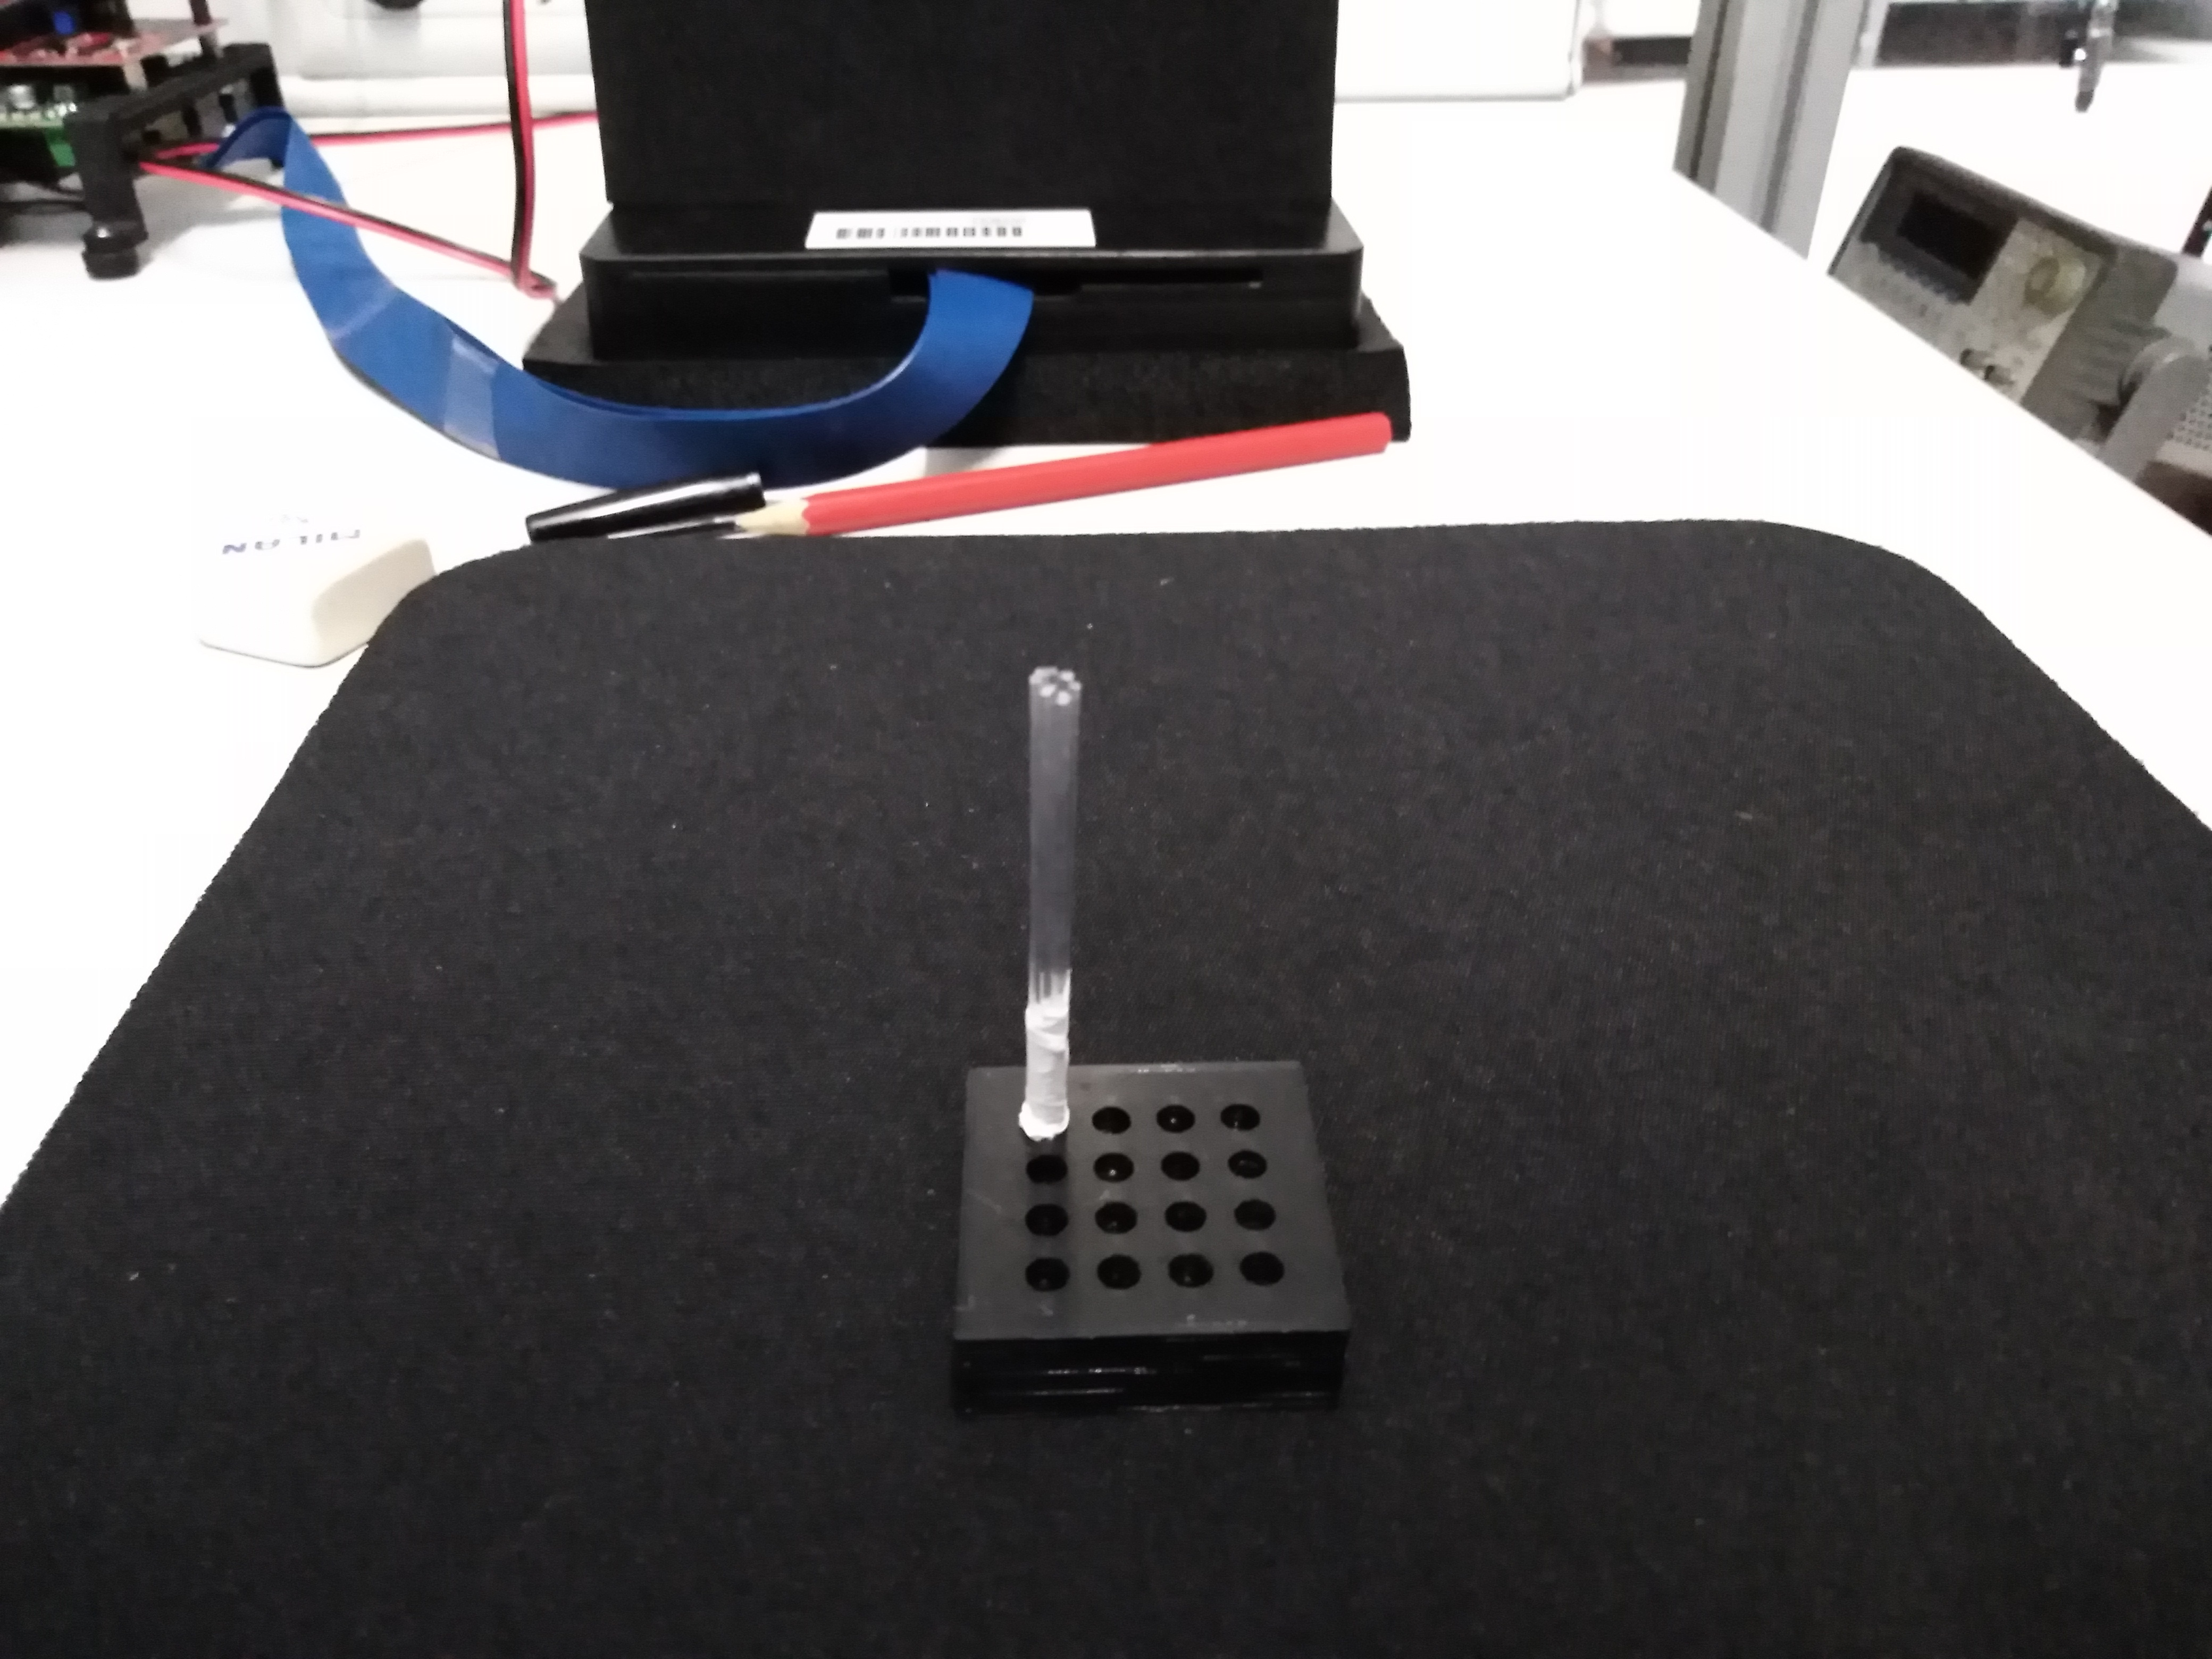
\includegraphics[scale=0.04]{PETSYS/Id_channel/3D_piece.jpg}
\caption{3D piece for identification each channel}
\end{figure}

\column{0.5\textwidth}

\begin{figure}[hbtp]
\centering
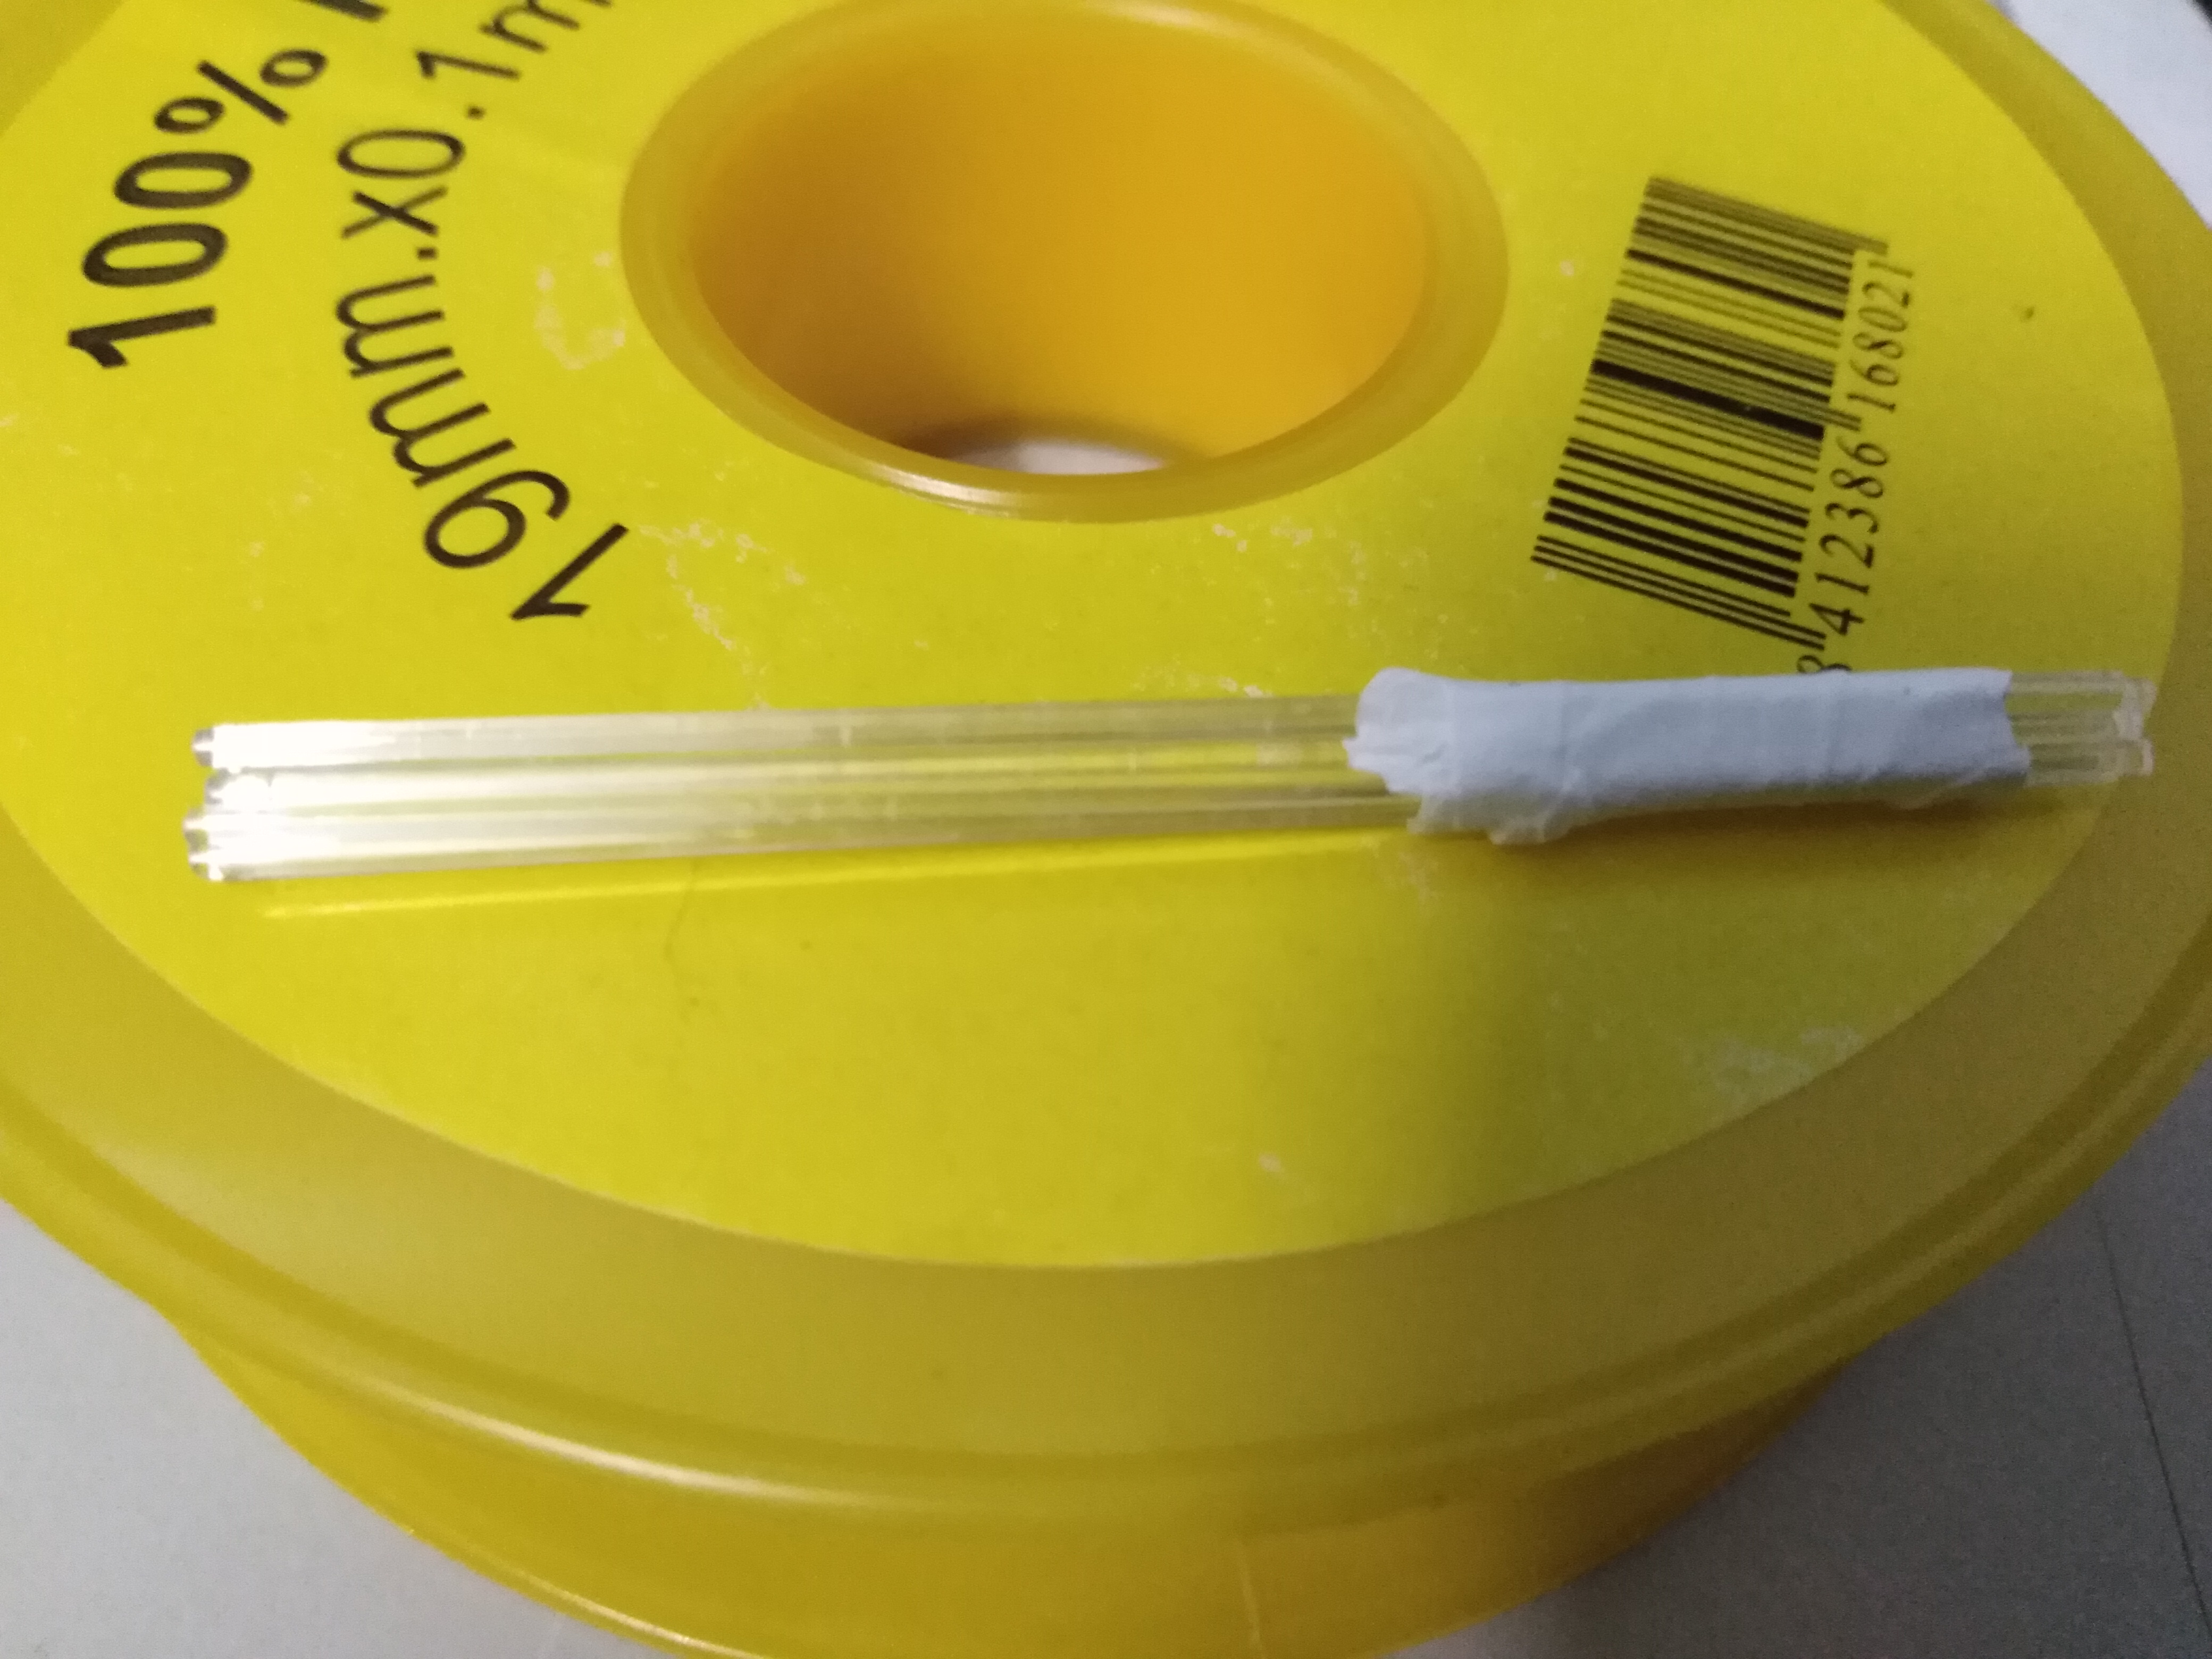
\includegraphics[scale=0.04]{PETSYS/Id_channel/Bunch_9_fibers.jpg}
\caption{Bunch with 9 fibers each one with 5 cm}
\end{figure}

\end{columns}

\end{itemize}

\end{frame}

\begin{frame}
\frametitle{PETSYS. Id. Channel}
\begin{itemize}
\item{}

\begin{figure}[hbtp]
\centering
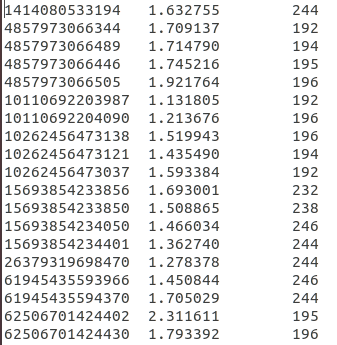
\includegraphics[scale=0.5]{PETSYS/Id_channel/Example_singles_PETSYS.png}
\caption{Example output single file}
\end{figure}

\end{itemize}

\end{frame}

\begin{frame}
\frametitle{PETSYS. Id. Channel}
\begin{itemize}
\item{} Pixel 1:

\begin{figure}[hbtp]
\centering
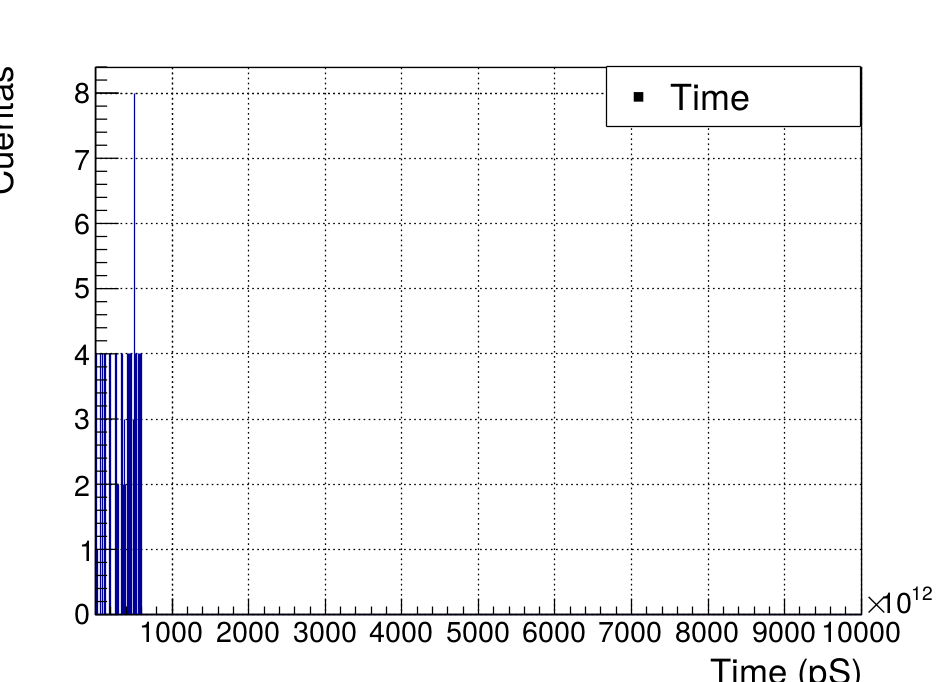
\includegraphics[scale=0.25]{PETSYS/Id_channel/time_spectrum_pixel_1.png}
\caption{Time spectrum}
\end{figure}

\end{itemize}

\end{frame}

\begin{frame}
\frametitle{PETSYS. Id. Channel}
\begin{itemize}
\item{} Pixel 1:

\begin{figure}[hbtp]
\centering
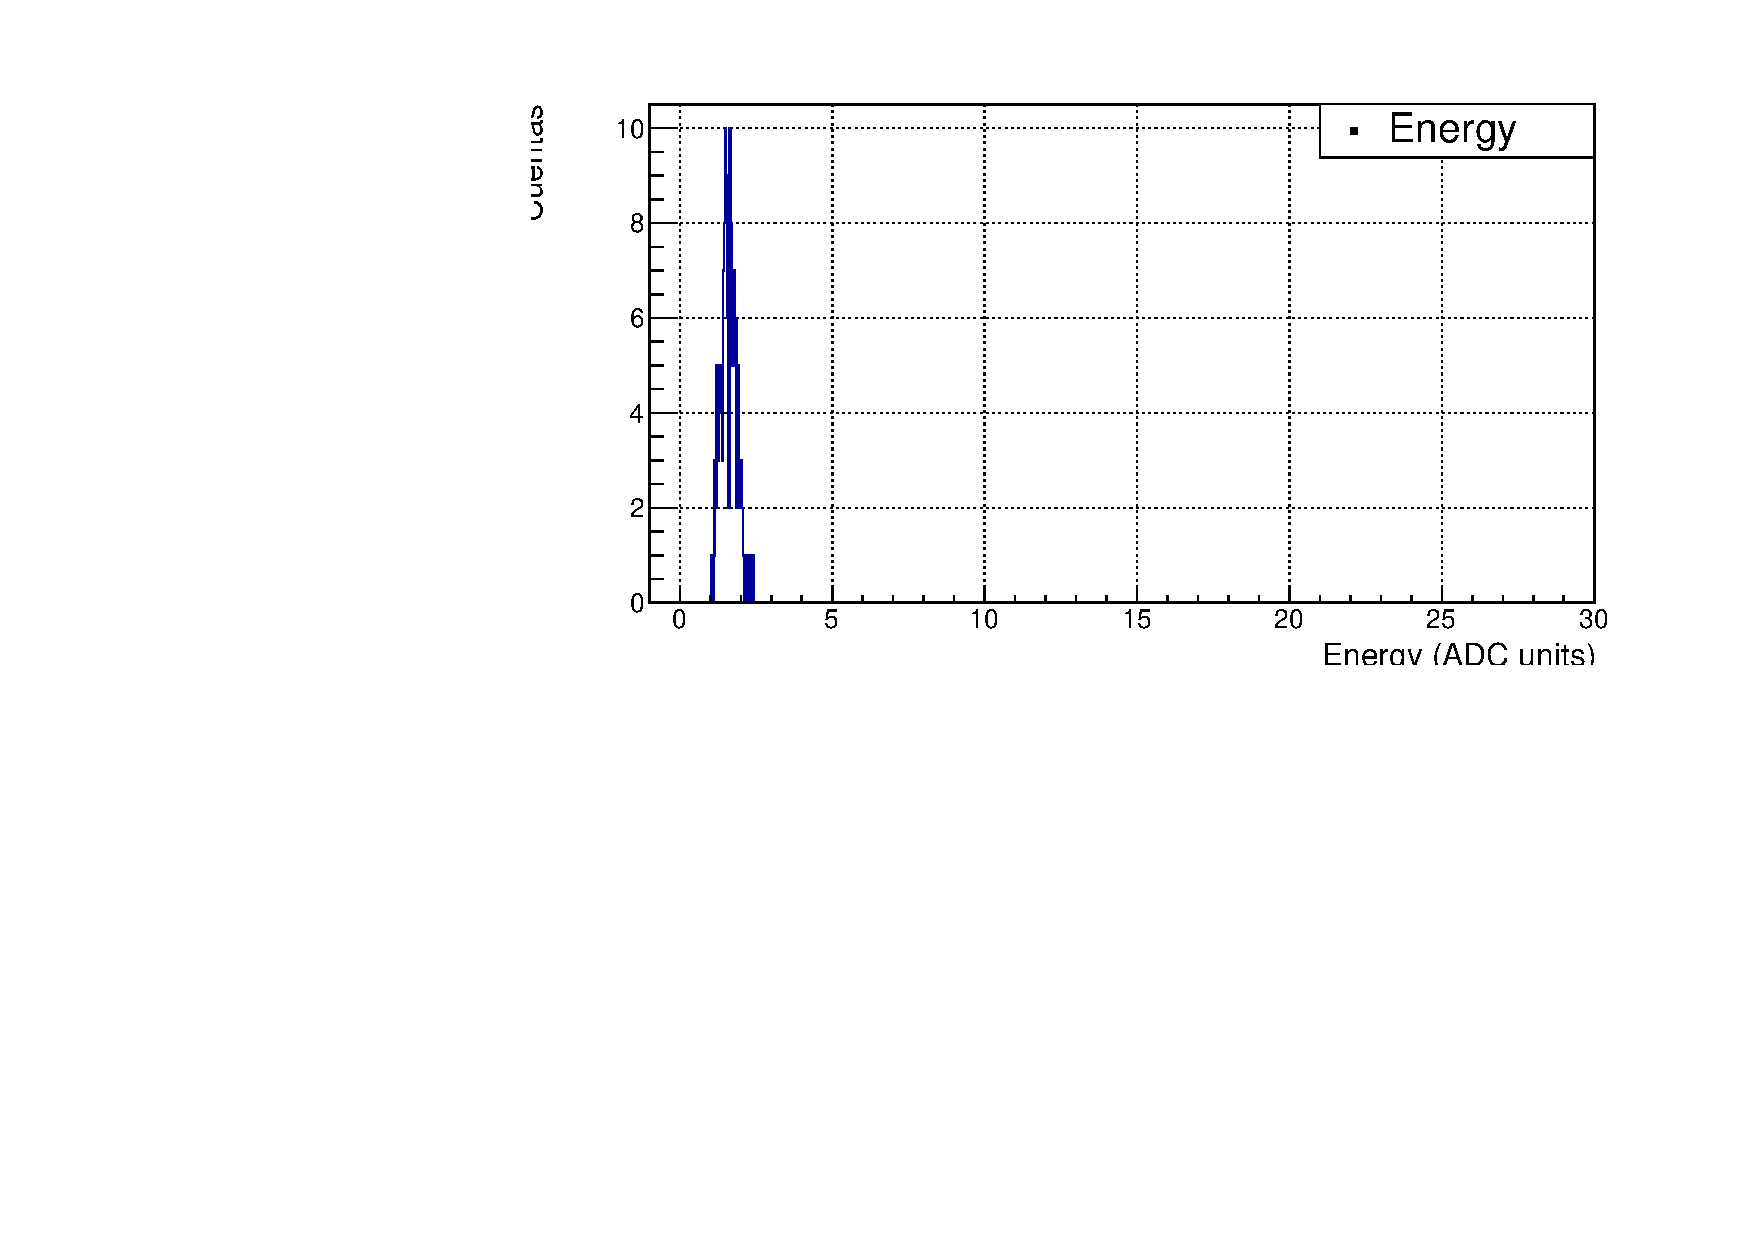
\includegraphics[scale=0.5]{PETSYS/Id_channel/energy_spectrum_pixel_1.pdf}
\caption{Energy spectrum}
\end{figure}

\end{itemize}

\end{frame}

\begin{frame}
\frametitle{PETSYS. Id. Channel}
\begin{itemize}
\item{} Pixel 1:

\begin{figure}[hbtp]
\centering
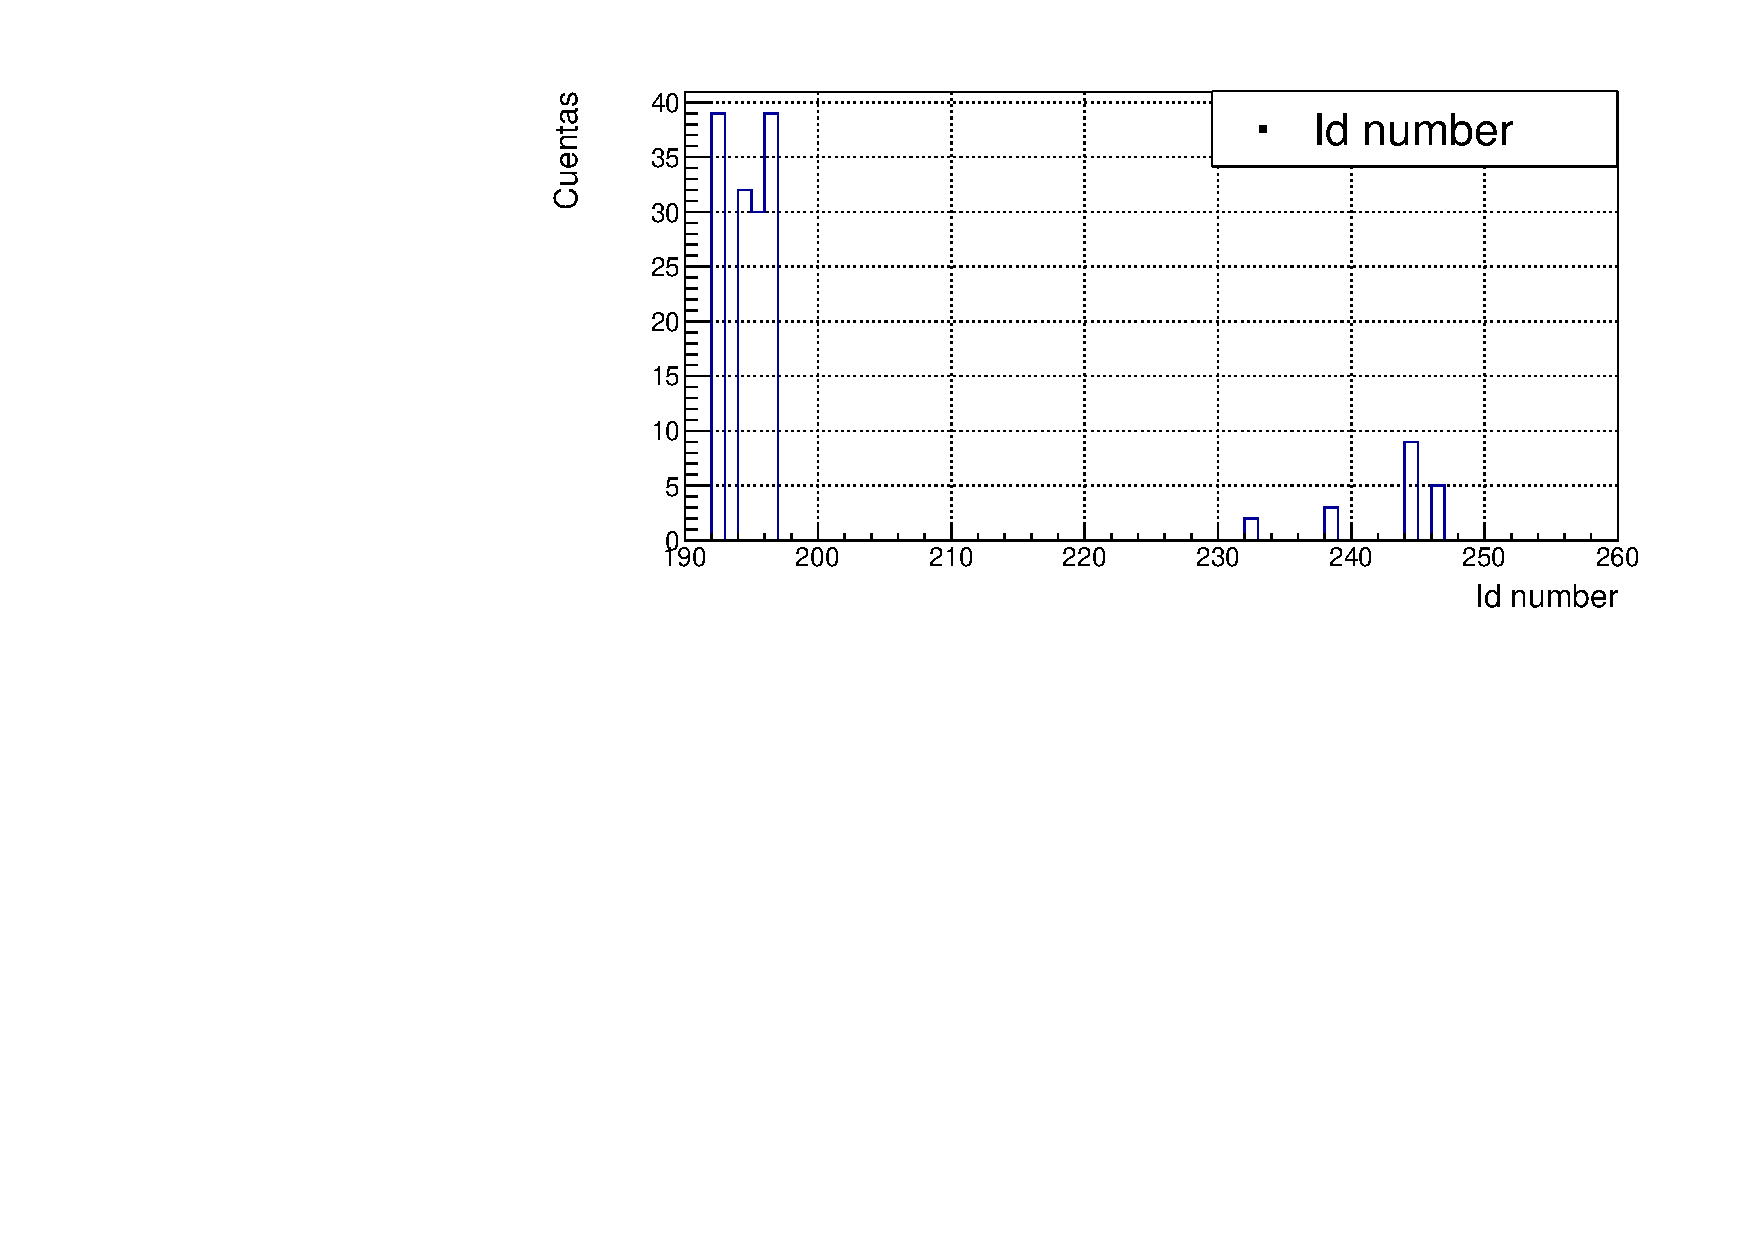
\includegraphics[scale=0.6]{PETSYS/Id_channel/Channel_pixel_1.pdf}
\caption{Channel histogram}
\end{figure}

\end{itemize}

\end{frame}

\begin{frame}
\frametitle{PETSYS. Id. Channel}
\begin{itemize}
\item{}

\begin{figure}[hbtp]
\centering
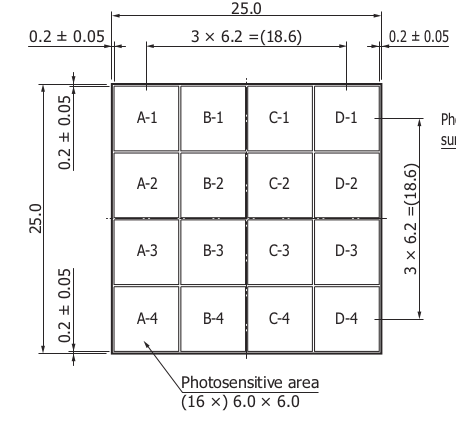
\includegraphics[scale=0.4]{PETSYS/Id_channel/Our_SIPM_schematic.png}
\caption{SiPM schematic}
\end{figure}

\end{itemize}

\end{frame}

\begin{frame}
\frametitle{PETSYS. Id. Channel}
\begin{itemize}
\item{}

\begin{figure}[hbtp]
\centering
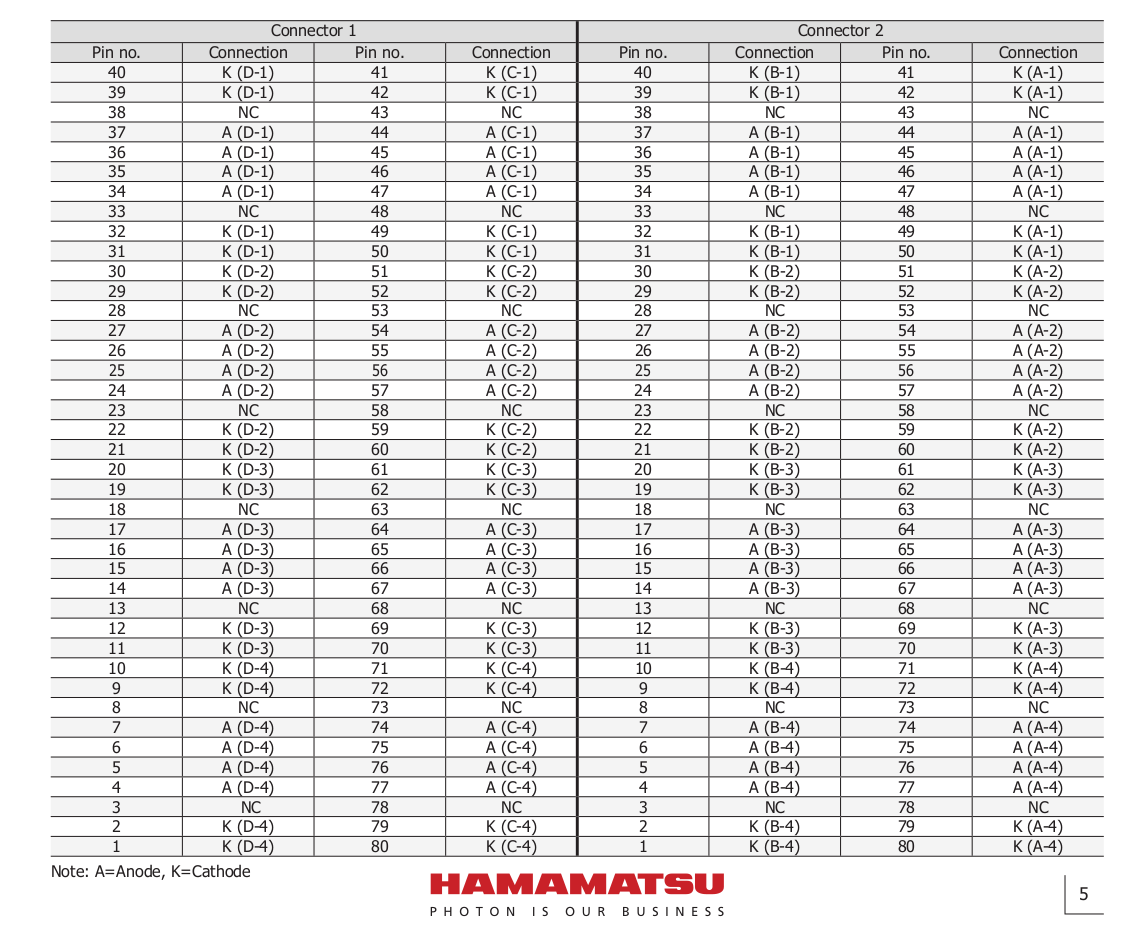
\includegraphics[scale=0.2]{PETSYS/Id_channel/relation_between_channels_and_SiPM.png}
\caption{Relation between channels and SiPMs}
\end{figure}

\end{itemize}

\end{frame}

\begin{frame}
\frametitle{PETSYS. Id. Channel}
\begin{itemize}
\item{} Pixel 1:

\begin{figure}[hbtp]
\centering
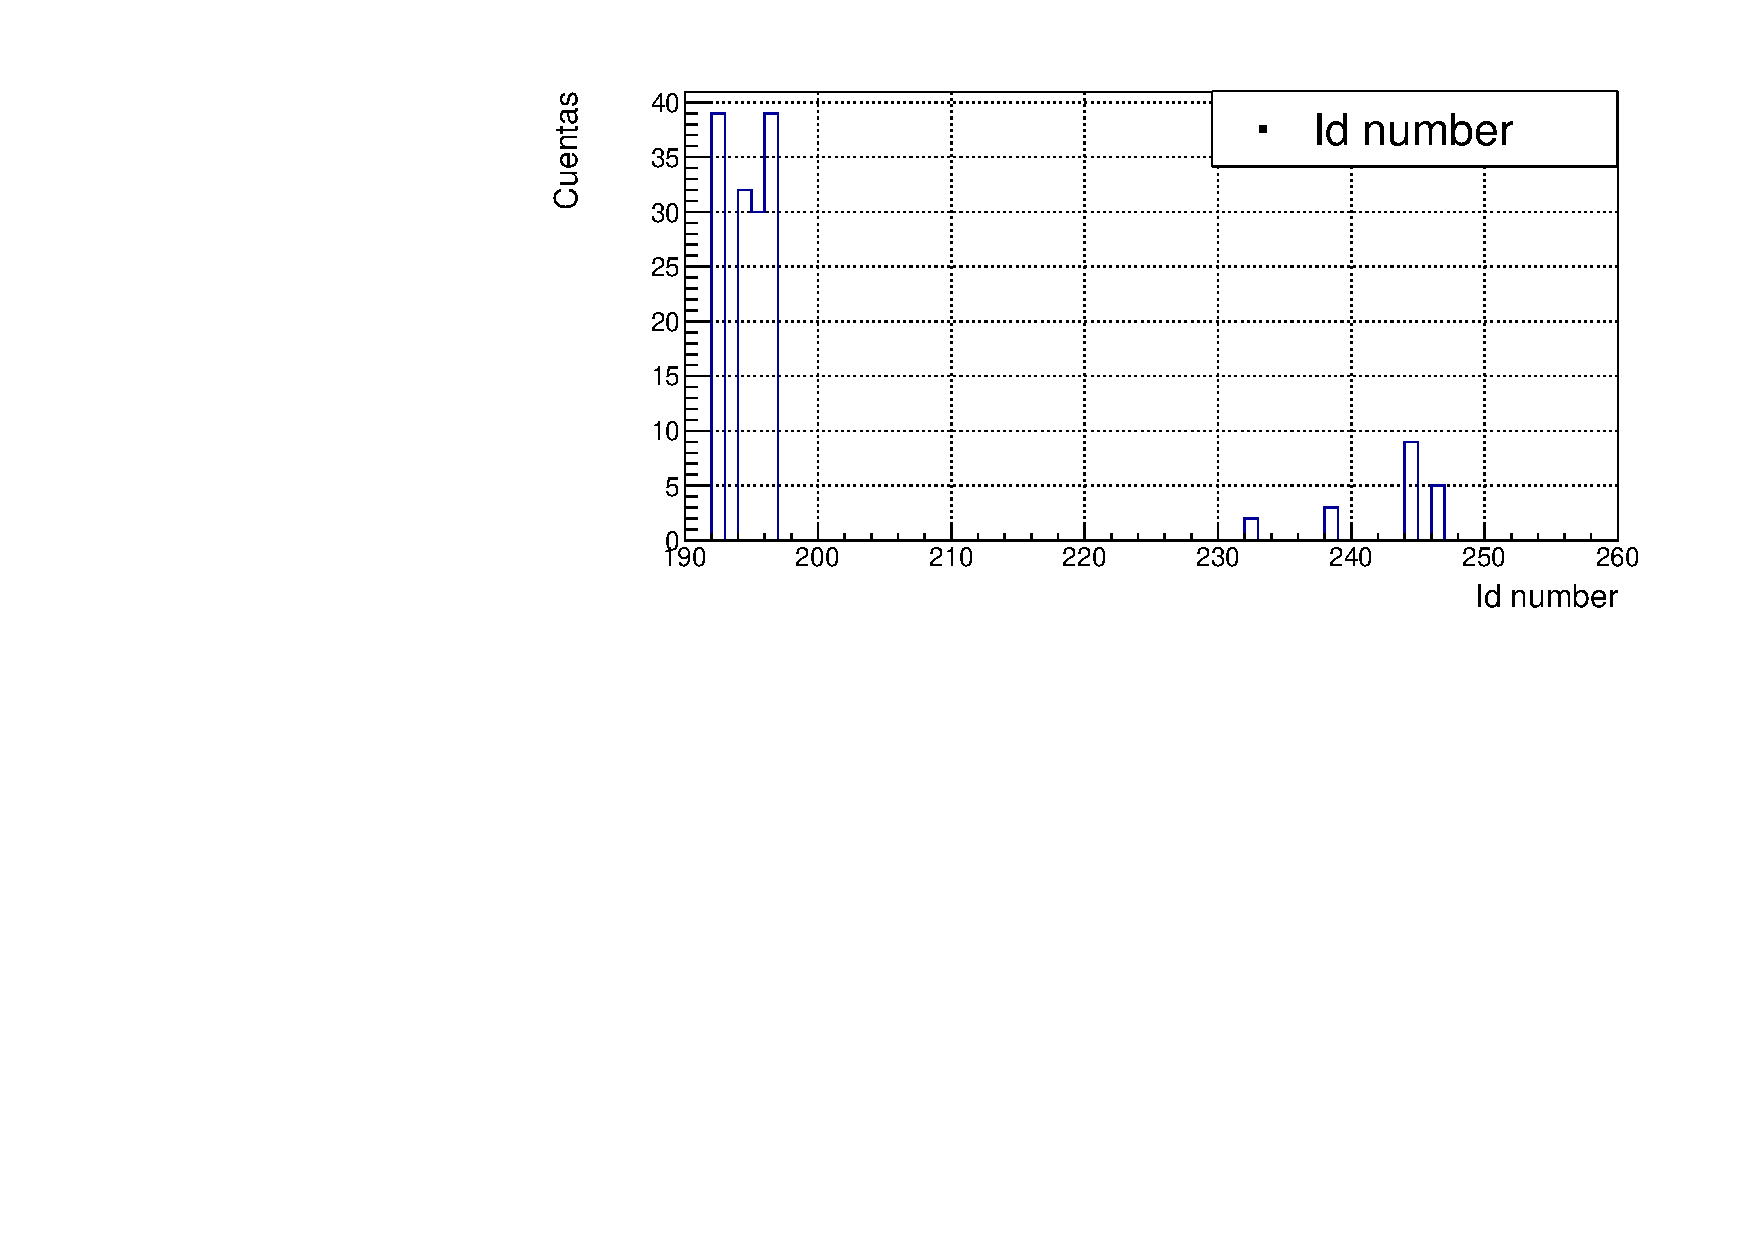
\includegraphics[scale=0.35]{PETSYS/Id_channel/Channel_pixel_1.pdf}
\caption{Channel histogram}
\end{figure}

\begin{block}{This system work}
We can identify the channel attached to each SiPM.
\end{block}

\end{itemize}

\end{frame}


\begin{frame}
\frametitle{PETSYS. Id. Channel}
\begin{itemize}
\item{} Pixel 1:

\begin{figure}[hbtp]
\centering
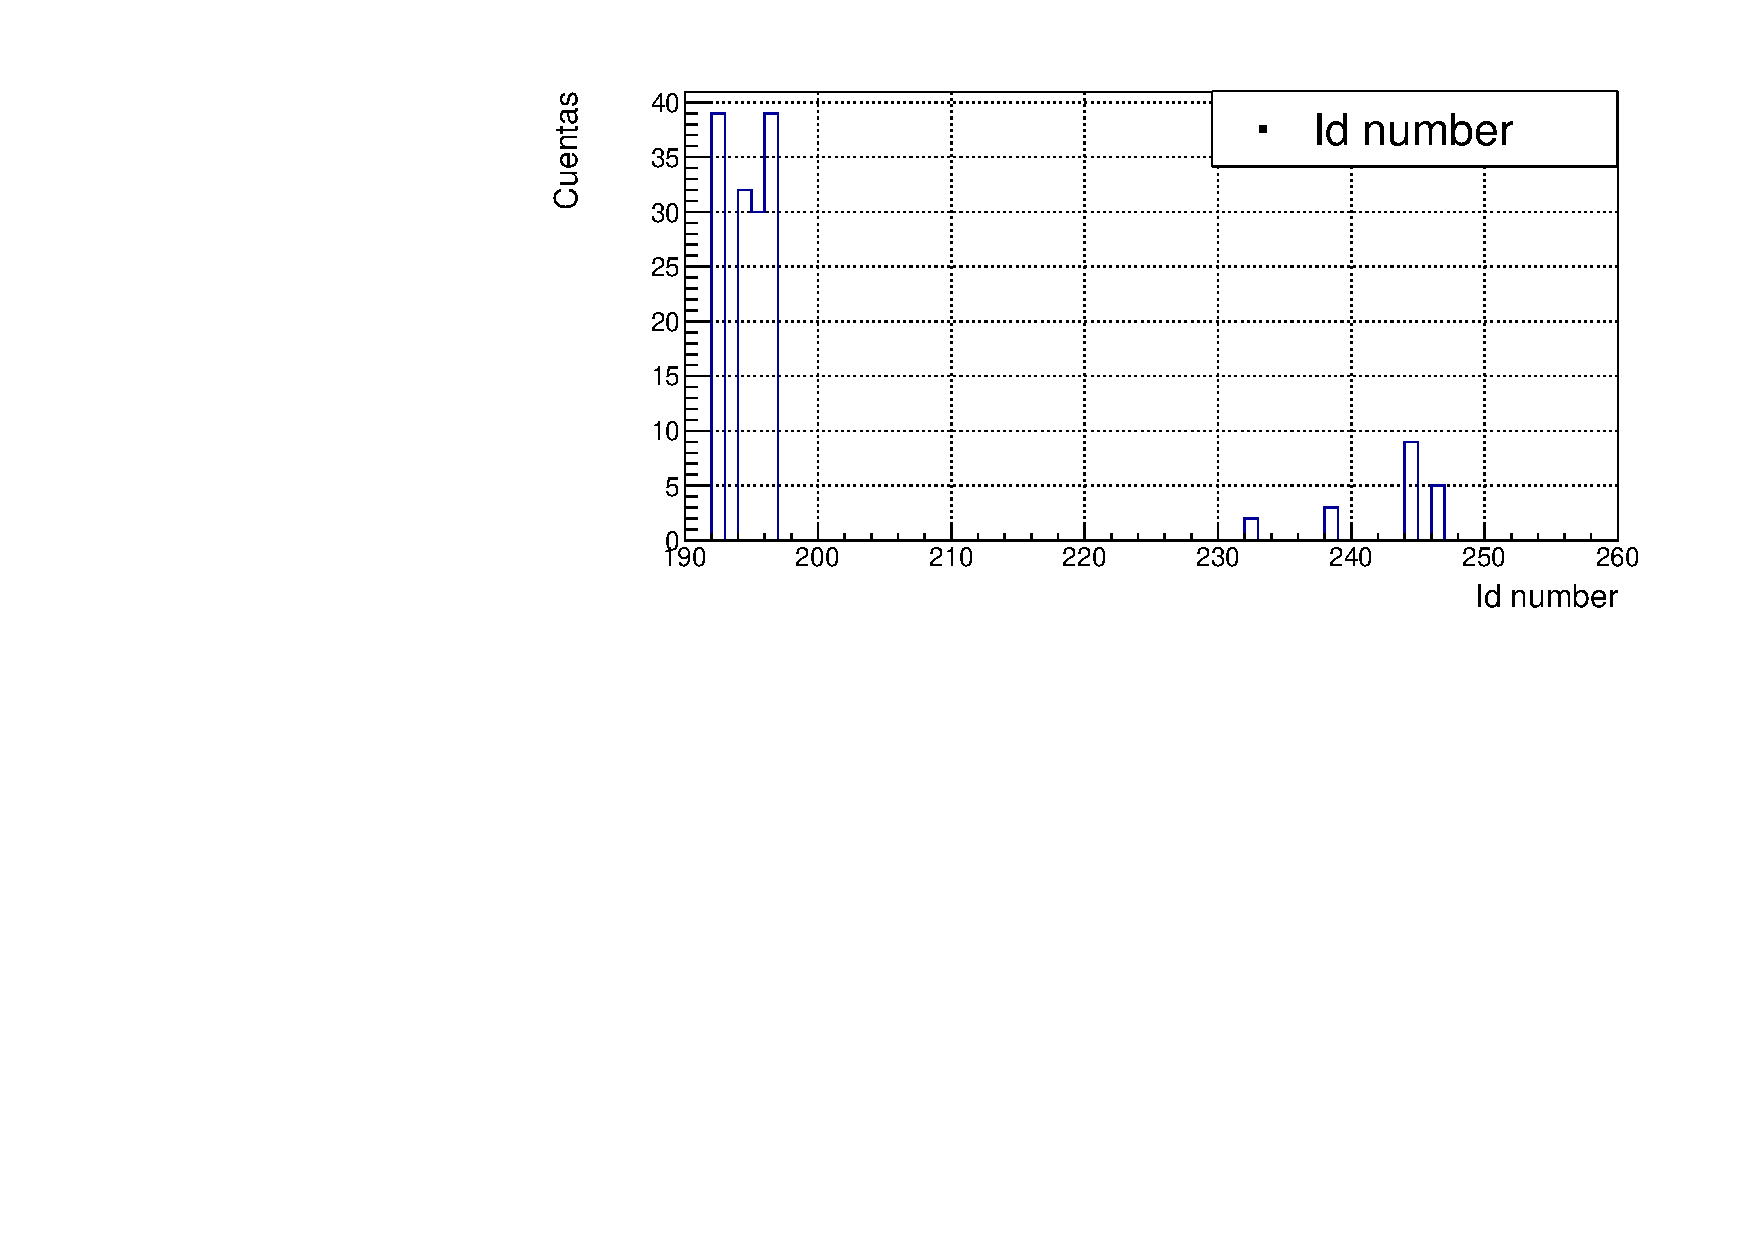
\includegraphics[scale=0.4]{PETSYS/Id_channel/Channel_pixel_1.pdf}
\caption{Channel histogram}
\end{figure}

\begin{alertblock}{Problem}
There is 1 channel, which correspond to the 15 SiPM, that has counts in all the cases.
\end{alertblock}

\end{itemize}

\end{frame}

\begin{frame}
\frametitle{PETSYS. Id. Channel}
\begin{itemize}
\item{} Channel identification:

\begin{table}
\begin{tabular}{l | c | c | c | c }
SiPM num. & Channel num. & SiPM num. & Channel num. \\
\hline \hline
1 & 192, 194, 195,196 & 9 & 236, 241, 247, 251 \\ 
2 & 193, 197, 199, 201 & 10 & 227, 231, 235, 237\\
3 & 198, 200, 206, 212 & 11 & 225, 229, 233, 239\\
4 & 202, 208, 214, 218 & 12 & 226, 230, 242, 243 \\
5 & 203, 205, 209, 216 & 13 & 248,250, 252, 254 \\ 
6 & 213, 215, 219, 221 & 14 & 245, 249, 253, 255 \\
7 & 207, 211, 217, 223 & 15 & 232, 238, 244, 246 \\
8 & 204, 210, 220, 222 & 16 & 224, 228, 234, 240   
\end{tabular}
\caption{Channel identification}
\end{table}

\end{itemize}

\end{frame}

\begin{frame}
\frametitle{PETSYS. Id. Channel}
\begin{itemize}
\item{} Channel identification: 
\begin{itemize}
\item{} Channels apparently messy.
\item{} I try to look for some relation between channels $\longrightarrow$ EXCEL
\end{itemize}

\end{itemize}

\end{frame}

\begin{frame}
\frametitle{PETSYS. Scintillator Crystal}
\begin{itemize}
\item{} I have disassambled and reassambled and I obtain this double peak again.
\begin{itemize}
	\item{} Emission spectrum of this crystal ($CaF_2$)
	\item{} Their size
\end{itemize}

\end{itemize}

\end{frame}



\begin{frame}
\frametitle{PETSYS. Polishing effect}

\begin{figure}[hbtp]
\centering
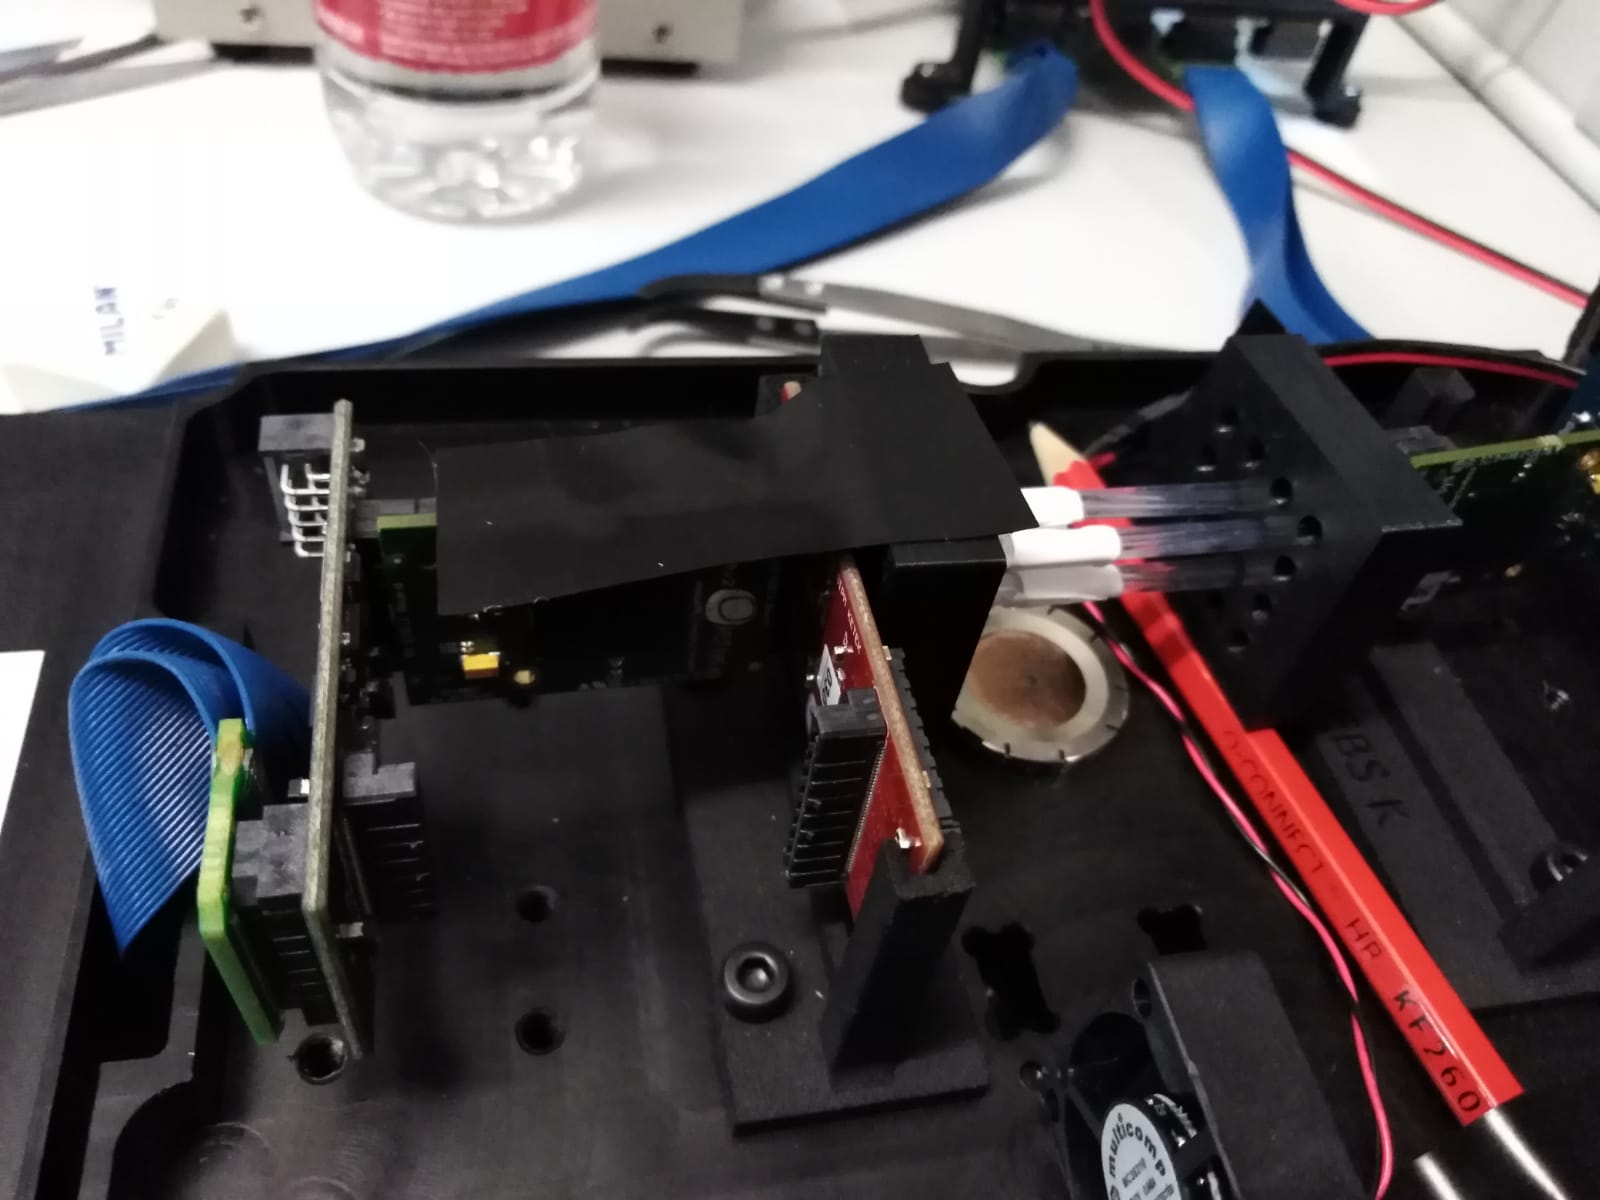
\includegraphics[scale=0.15]{PETSYS/Polishing_effect/Set_up_polishing.jpeg}
\caption{4 bunch with 8 fibers each one. Pixels 6, 7, 10, 11}
\end{figure}

\end{frame}

\begin{frame}
\frametitle{PETSYS. Other posible studies}

\begin{itemize}
\item{} I have cutted and polished near to 600 fibers of 5 mm.
\item{} Any idea?
\end{itemize}

\end{frame}

\begin{frame}
\frametitle{LARAM. Polishing effect with PMTs}

\begin{figure}[hbtp]
\centering
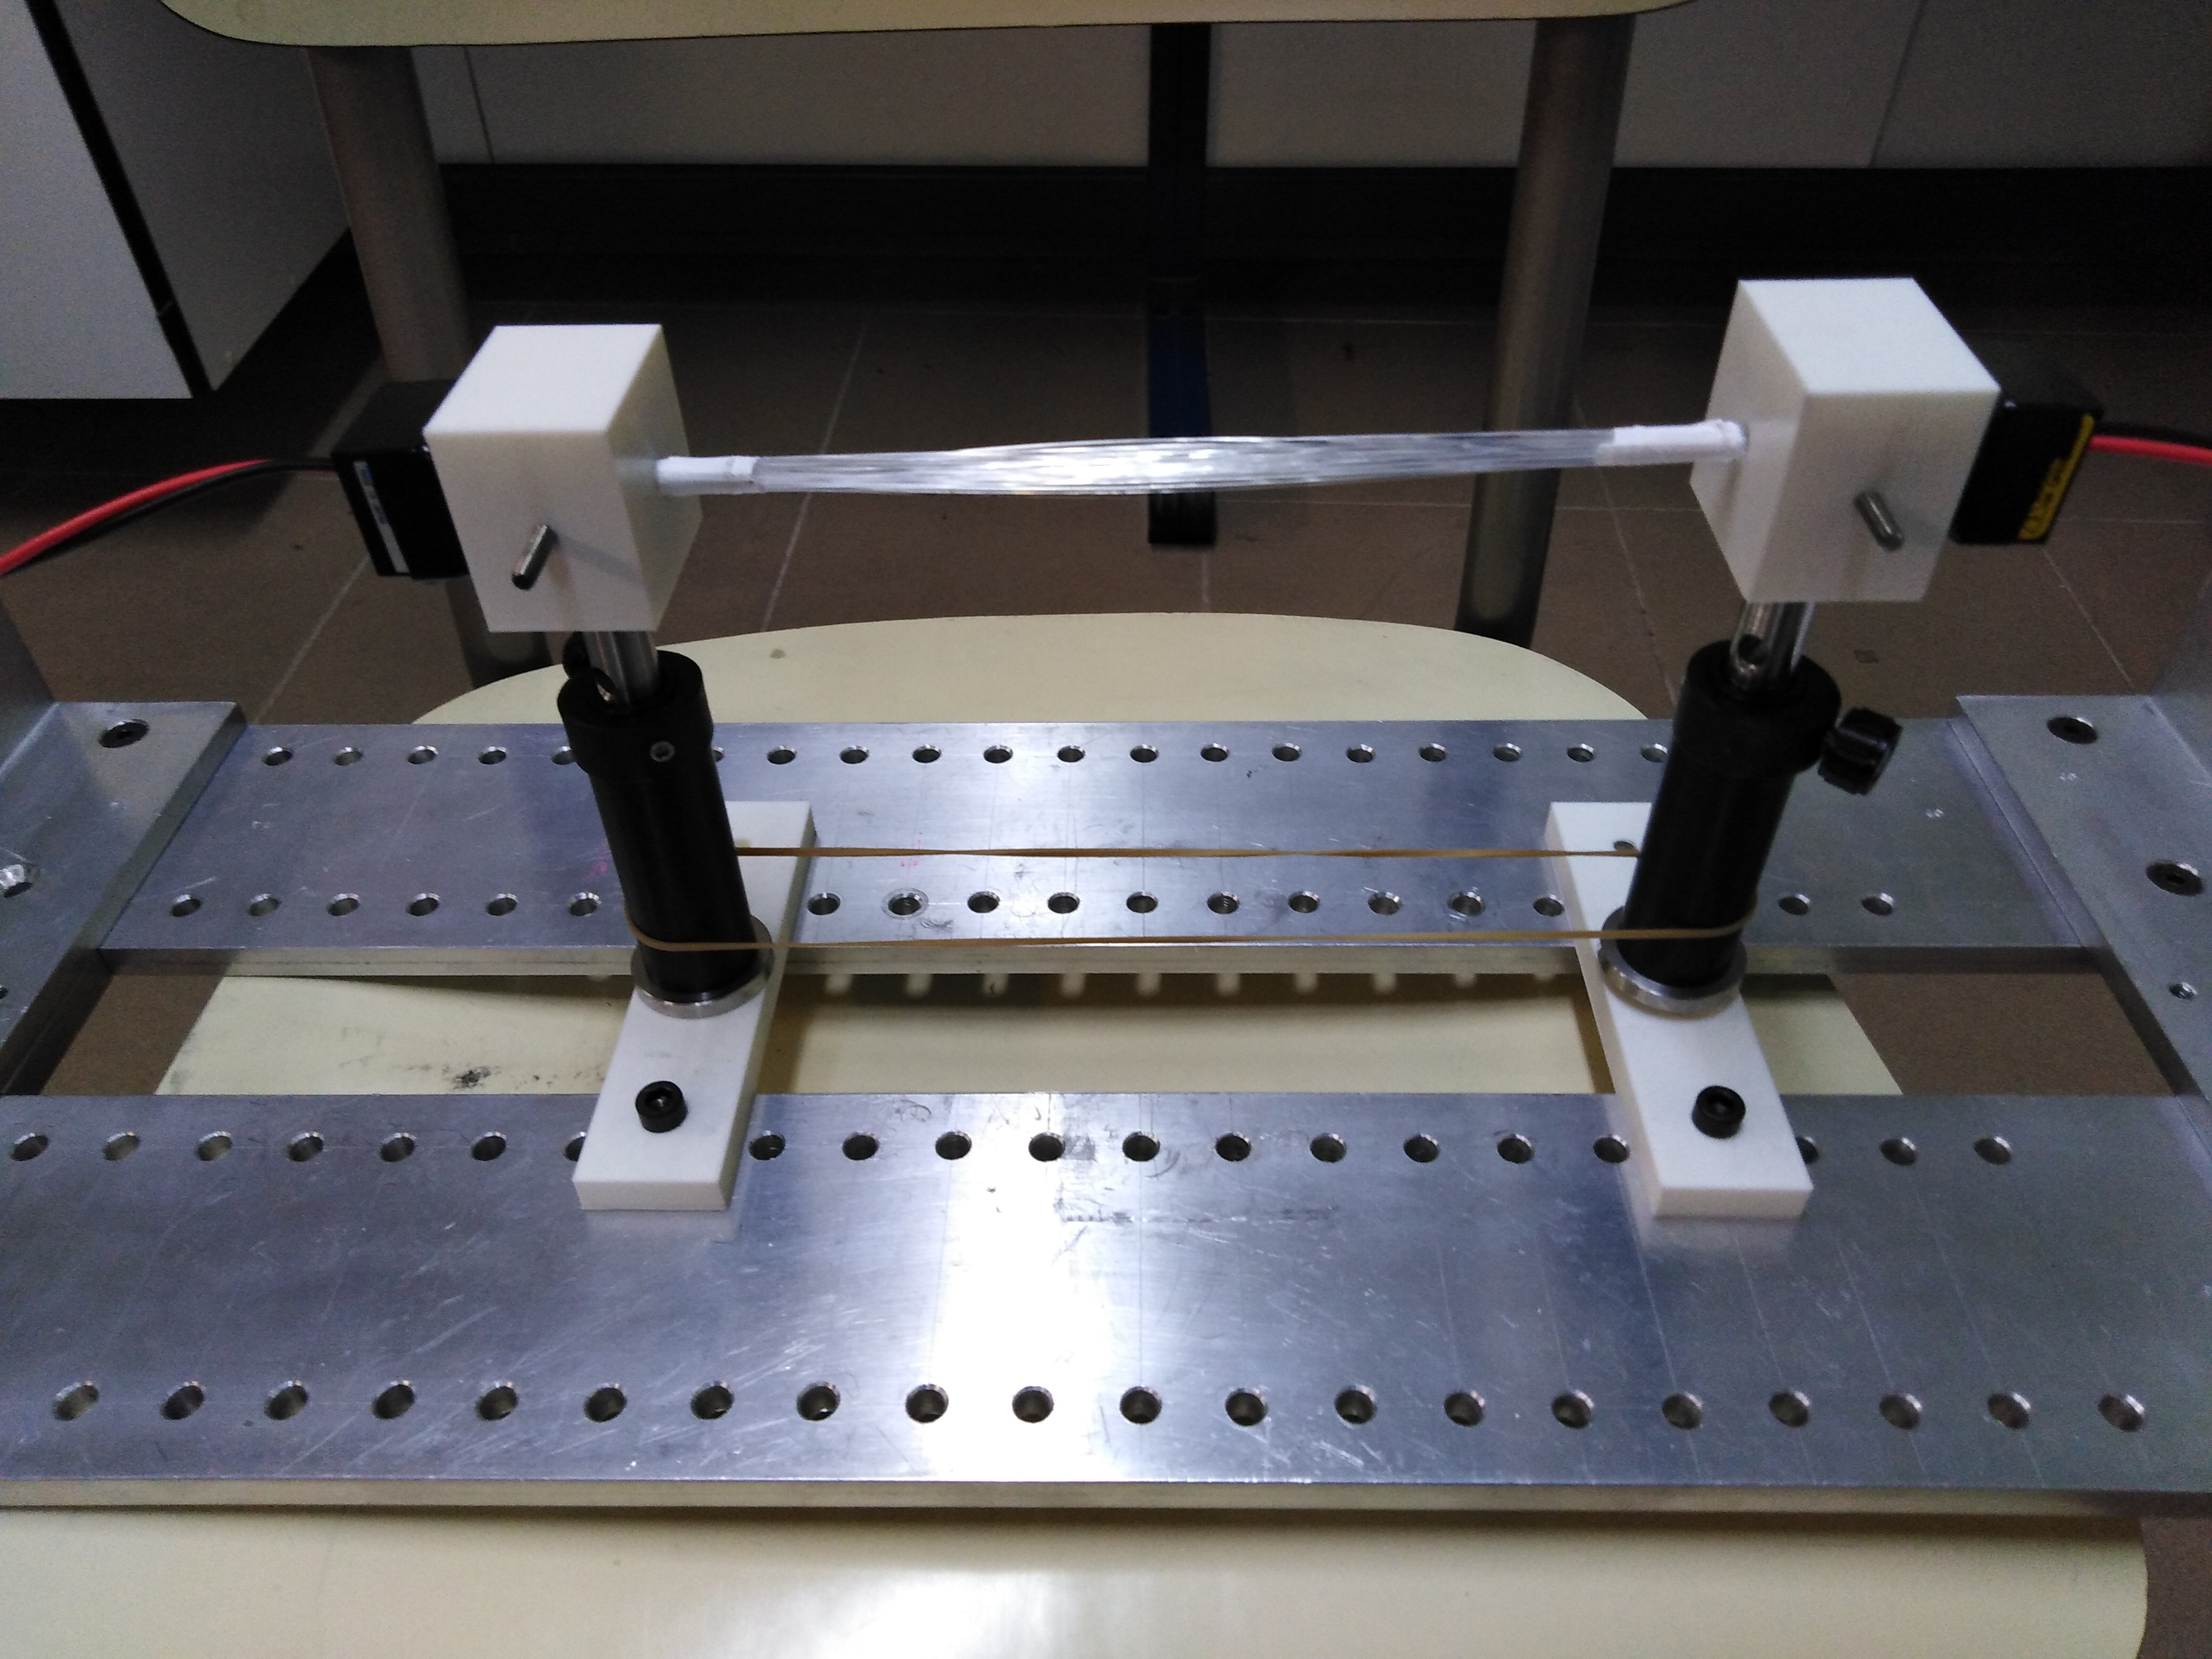
\includegraphics[scale=0.06]{LARAM/Polishing_effect/Set_up_polish_LARAM.jpg}
\caption{Bunch with 25 fibers with 15 cm}
\end{figure}

\end{frame}



\begin{frame}
\frametitle{LARAM. Polishing effect with PMTs}
First try

\begin{columns}
\column{0.5\textwidth}

\begin{figure}[hbtp]
\centering
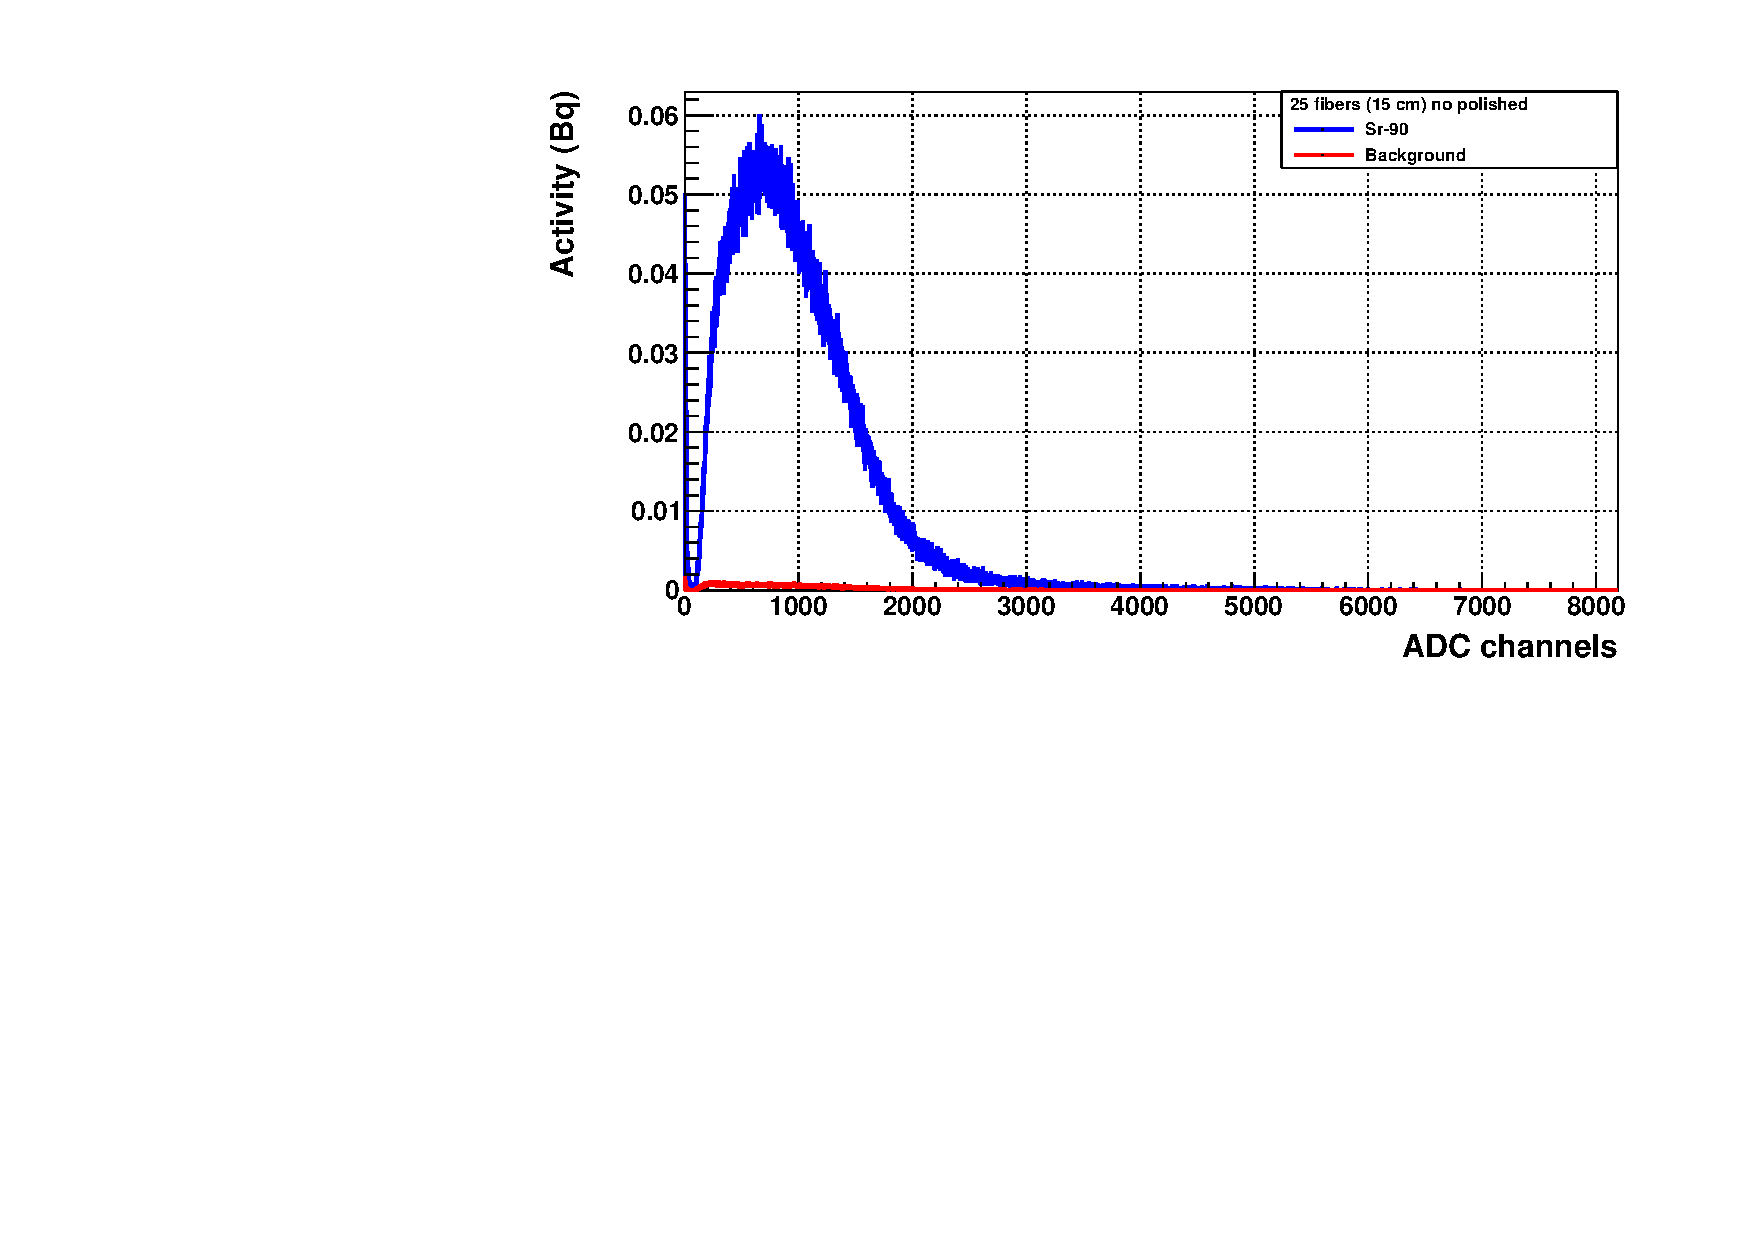
\includegraphics[scale=0.3]{LARAM/Polishing_effect/First_try/No_polished/Sr_90_background.pdf}
\caption{Sr-90 with fibers not polished}
\end{figure}

\column{0.5\textwidth}

\begin{figure}[hbtp]
\centering
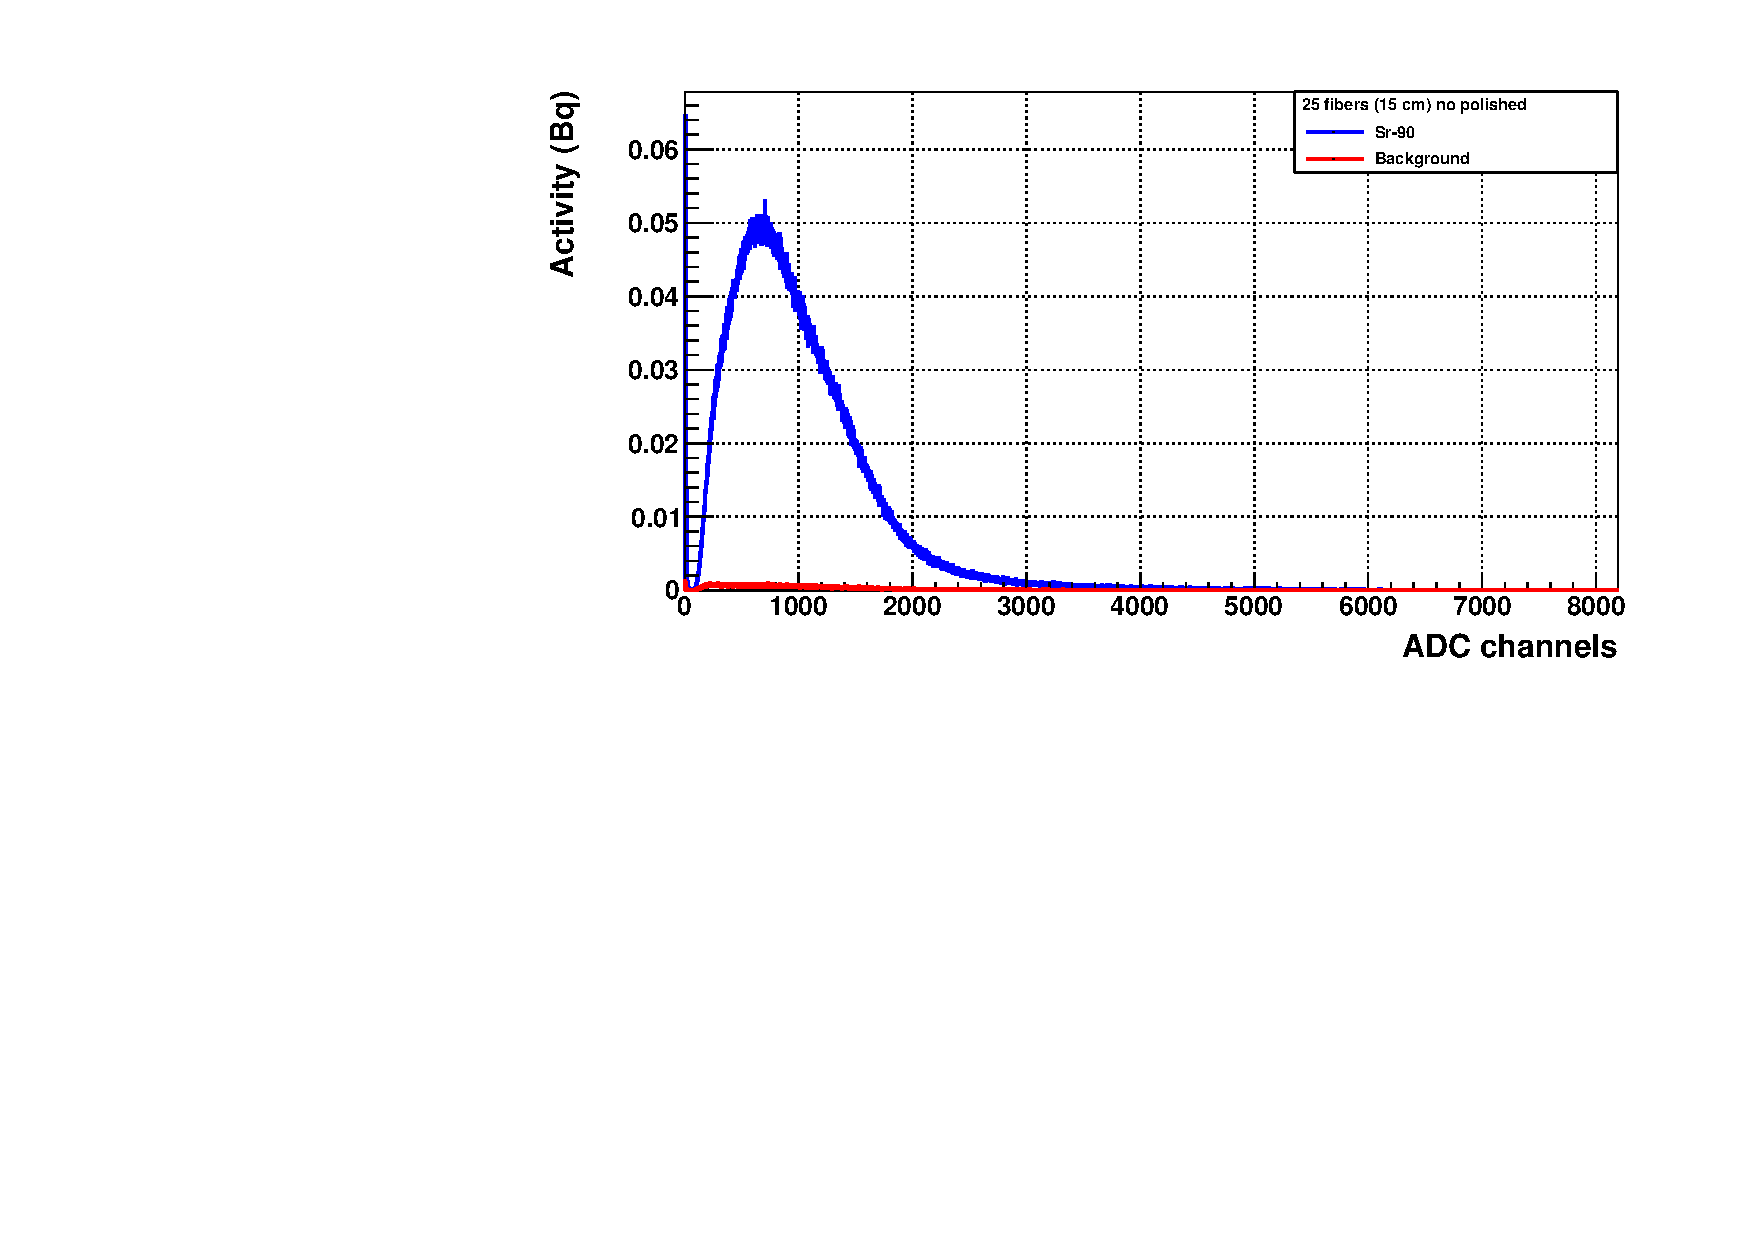
\includegraphics[scale=0.3]{LARAM/Polishing_effect/First_try/Polished/Sr_90_background.pdf}
\caption{Sr-90 with fibers polished}
\end{figure}

\end{columns}

\end{frame}


\begin{frame}
\frametitle{LARAM. Polishing effect with PMTs}
First try\\

\begin{columns}
\column{0.5\textwidth}

\begin{figure}[hbtp]
\centering
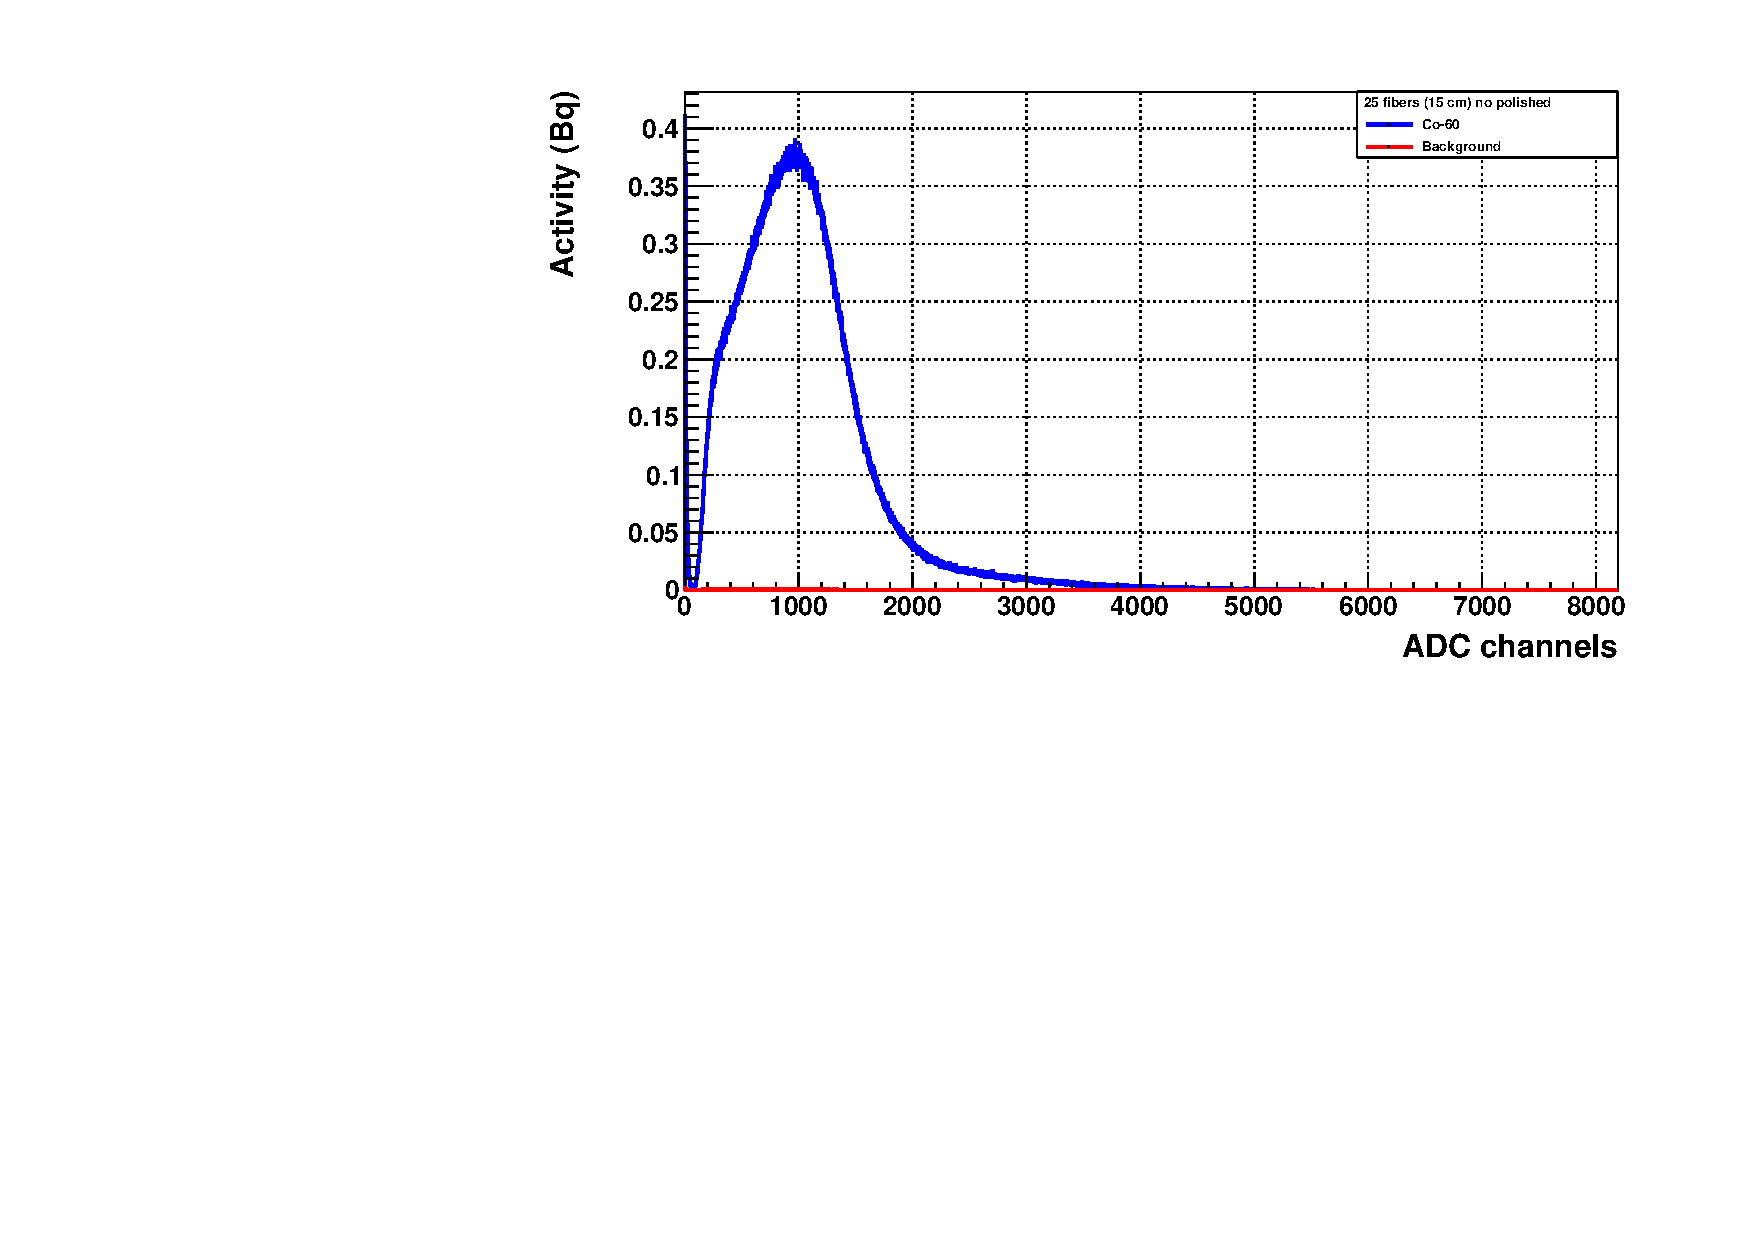
\includegraphics[scale=0.3]{LARAM/Polishing_effect/First_try/No_polished/Co_60_background.pdf}
\caption{Co-60 with fibers not polished}
\end{figure}

\column{0.5\textwidth}

\begin{figure}[hbtp]
\centering
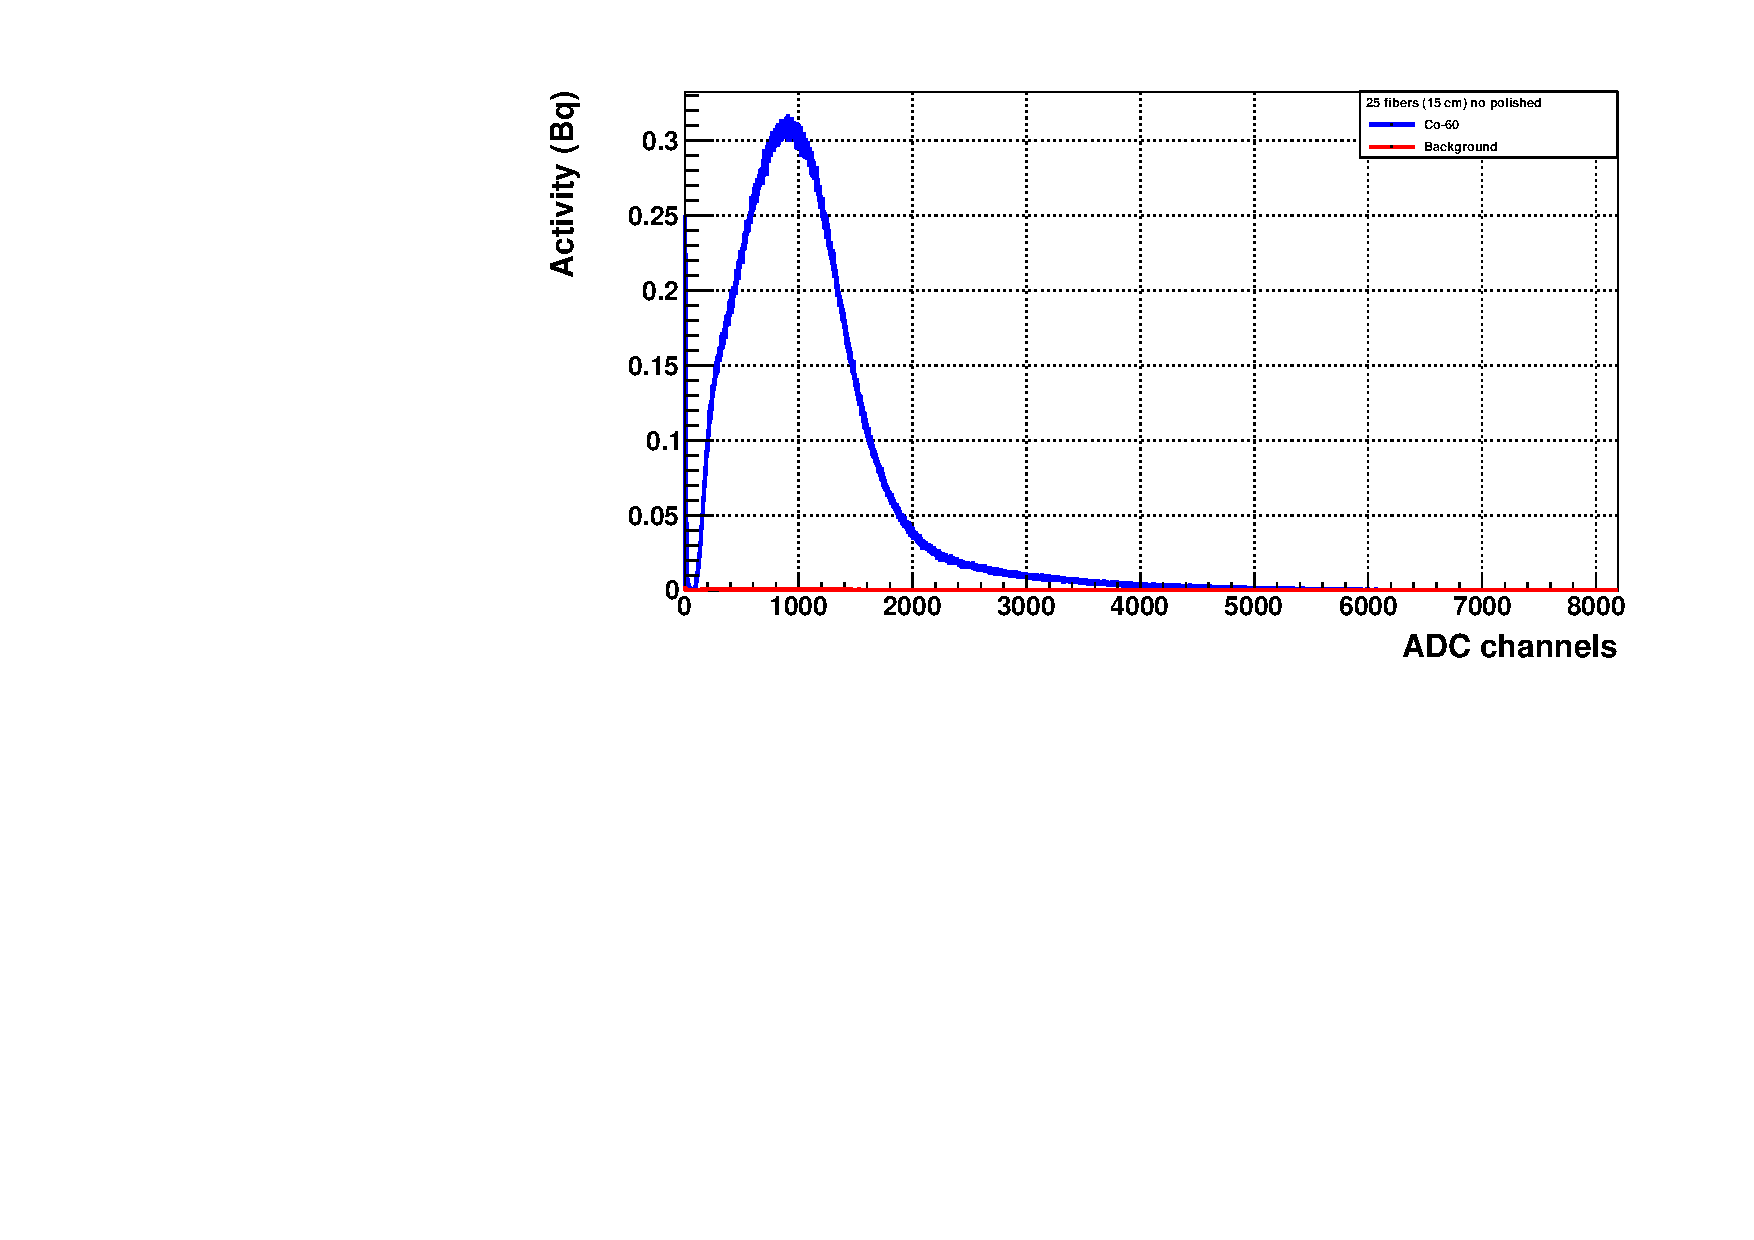
\includegraphics[scale=0.3]{LARAM/Polishing_effect/First_try/Polished/Co_60_background.pdf}
\caption{Co-60 with fibers polished}
\end{figure}

\end{columns}

\end{frame}

\begin{frame}
\frametitle{LARAM. Polishing effect with PMTs}
First try

\begin{figure}[hbtp]
\centering
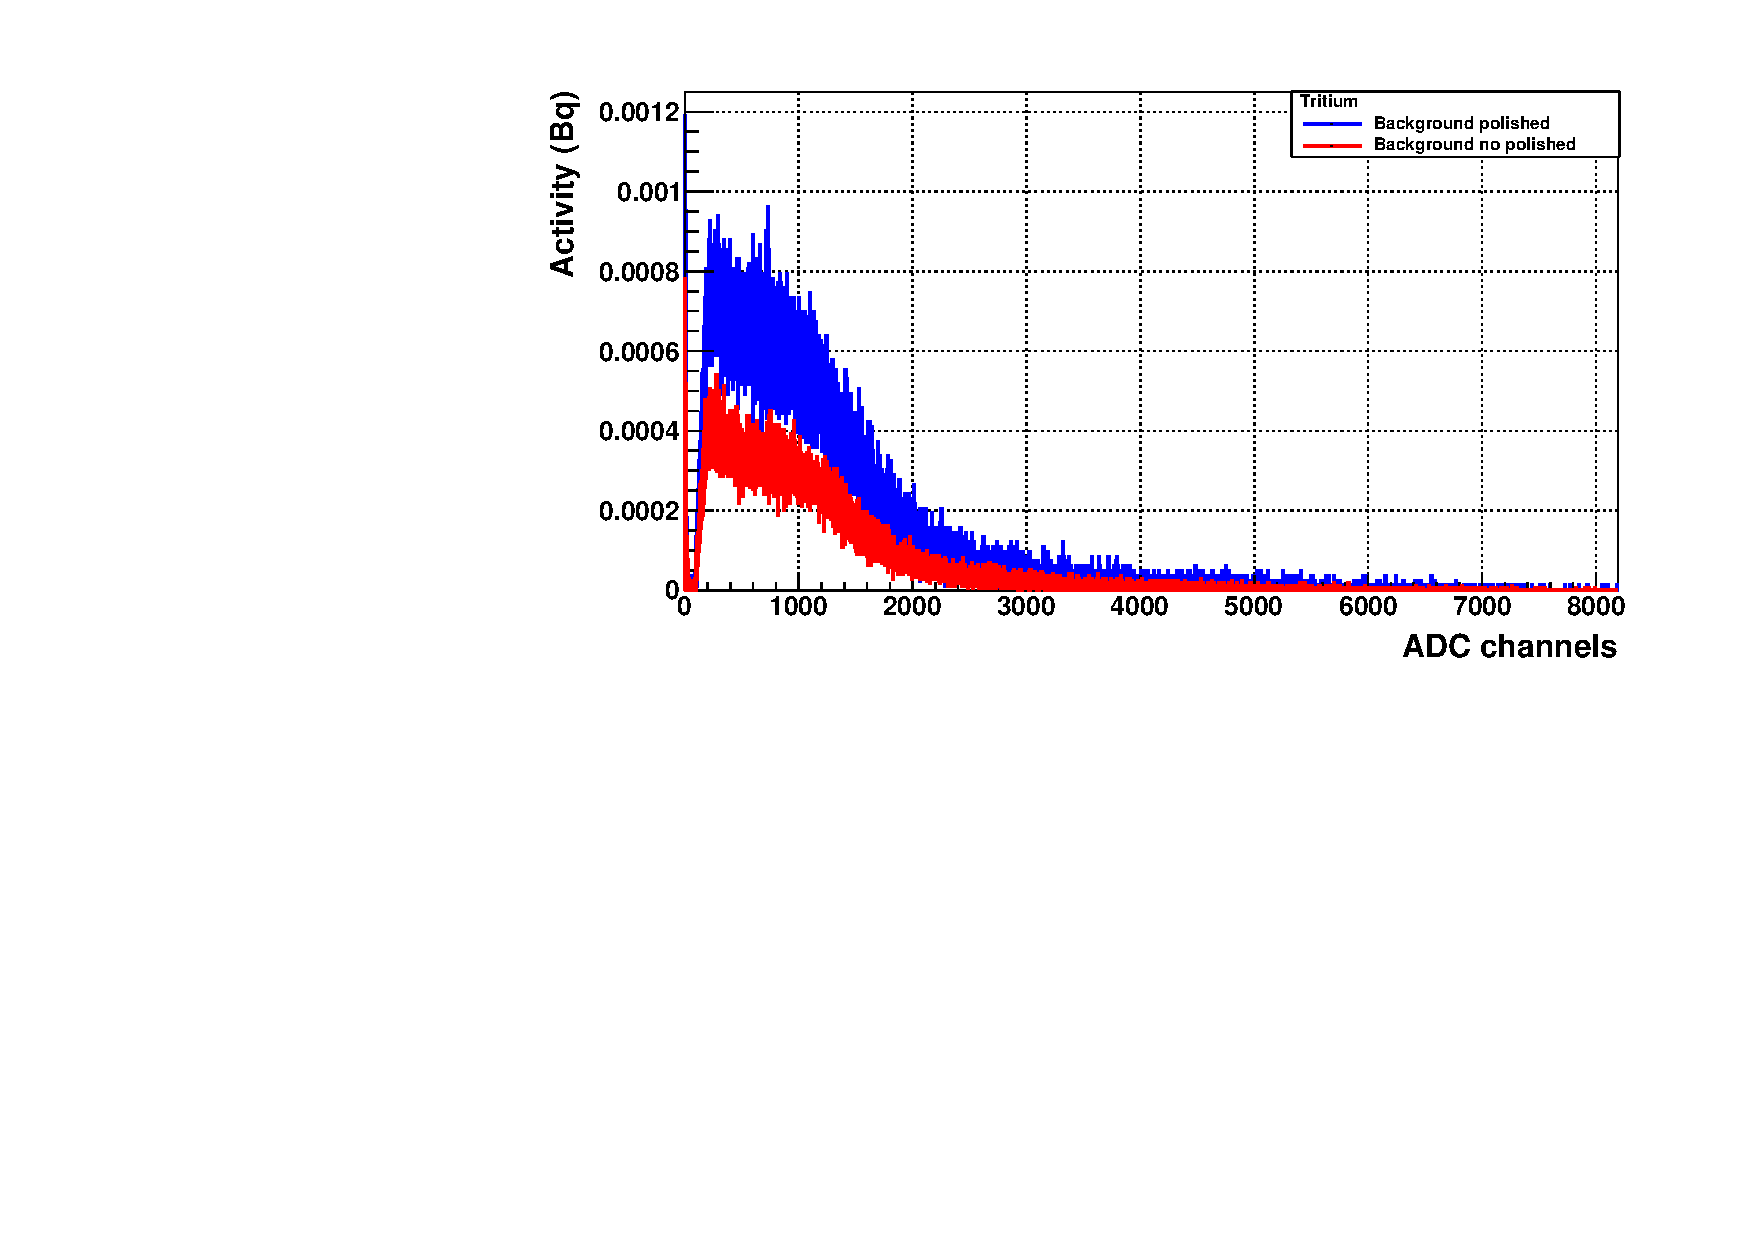
\includegraphics[scale=0.5]{LARAM/Polishing_effect/First_try/Background_polish_not_polish.pdf}
\caption{Bunch with 25 fibers with 15 cm}
\end{figure}

\end{frame}

\begin{frame}
\frametitle{LARAM. Polishing effect with PMTs}
Second try (same bunch)

\begin{columns}
\column{0.5\textwidth}

\begin{figure}[hbtp]
\centering
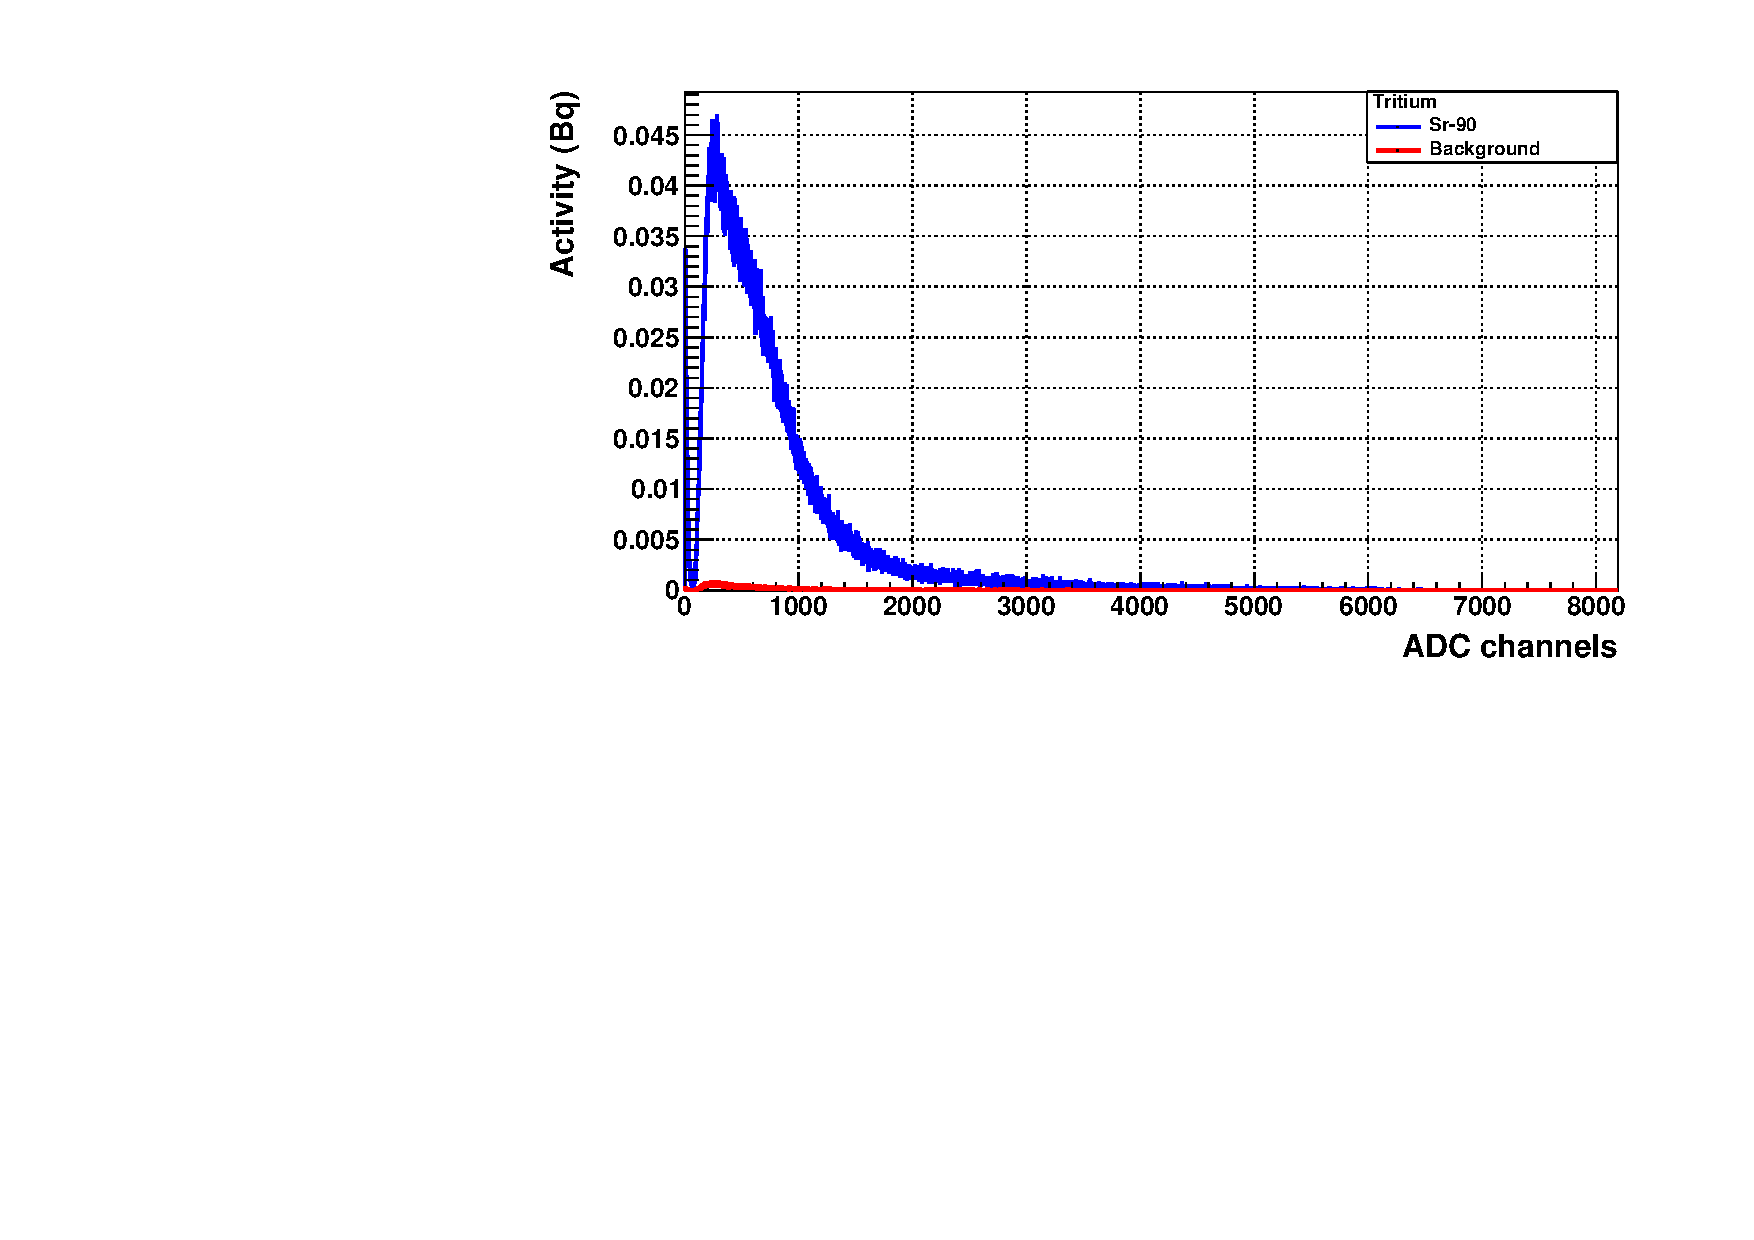
\includegraphics[scale=0.3]{LARAM/Polishing_effect/Second_try/No_polished/Sr_90_no_polished.pdf}
\caption{Sr-90 with fibers not polished}
\end{figure}

\column{0.5\textwidth}

\begin{figure}[hbtp]
\centering
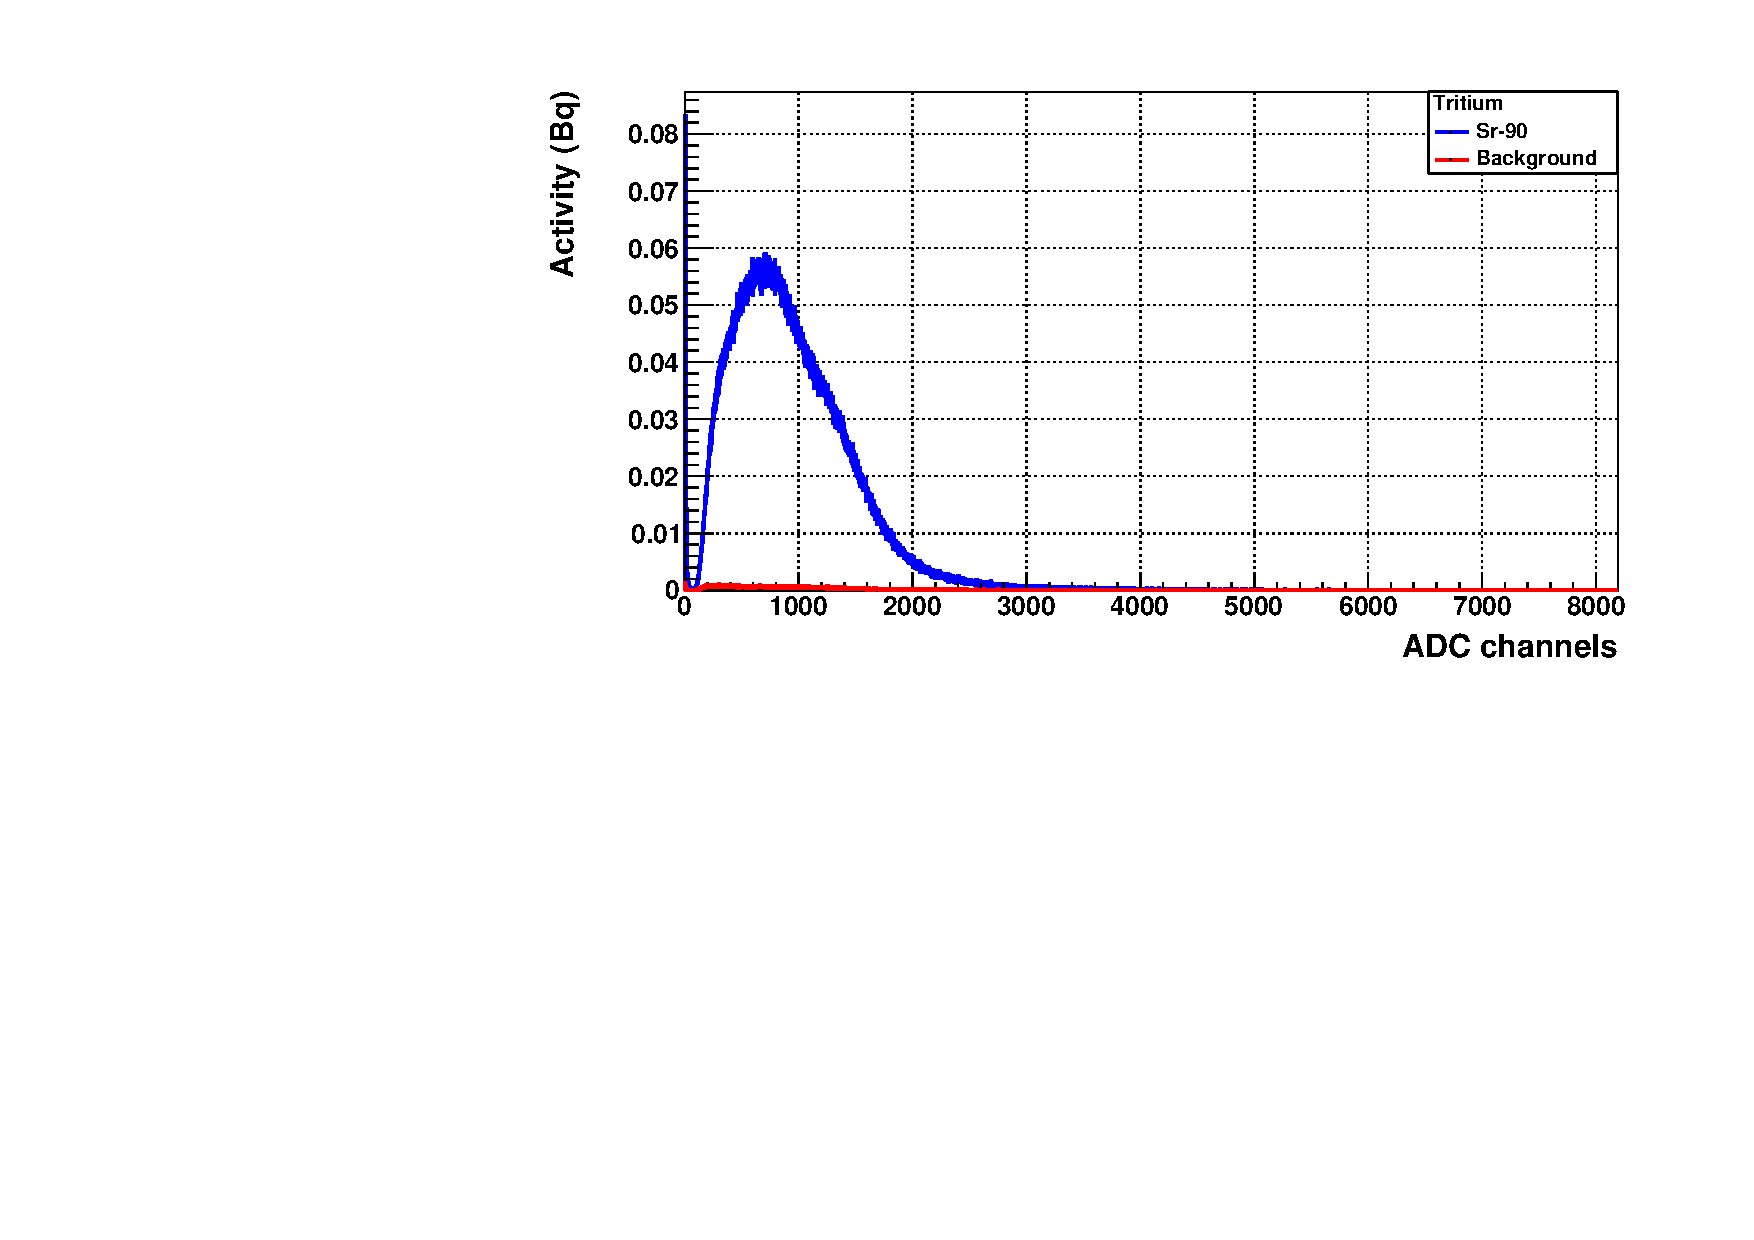
\includegraphics[scale=0.3]{LARAM/Polishing_effect/Second_try/Polished/Sr_90_polished.pdf}
\caption{Sr-90 with fibers polished}
\end{figure}

\end{columns}

\end{frame}


\begin{frame}
\frametitle{LARAM. Polishing effect with PMTs}
Second try\\

\begin{columns}
\column{0.5\textwidth}

\begin{figure}[hbtp]
\centering
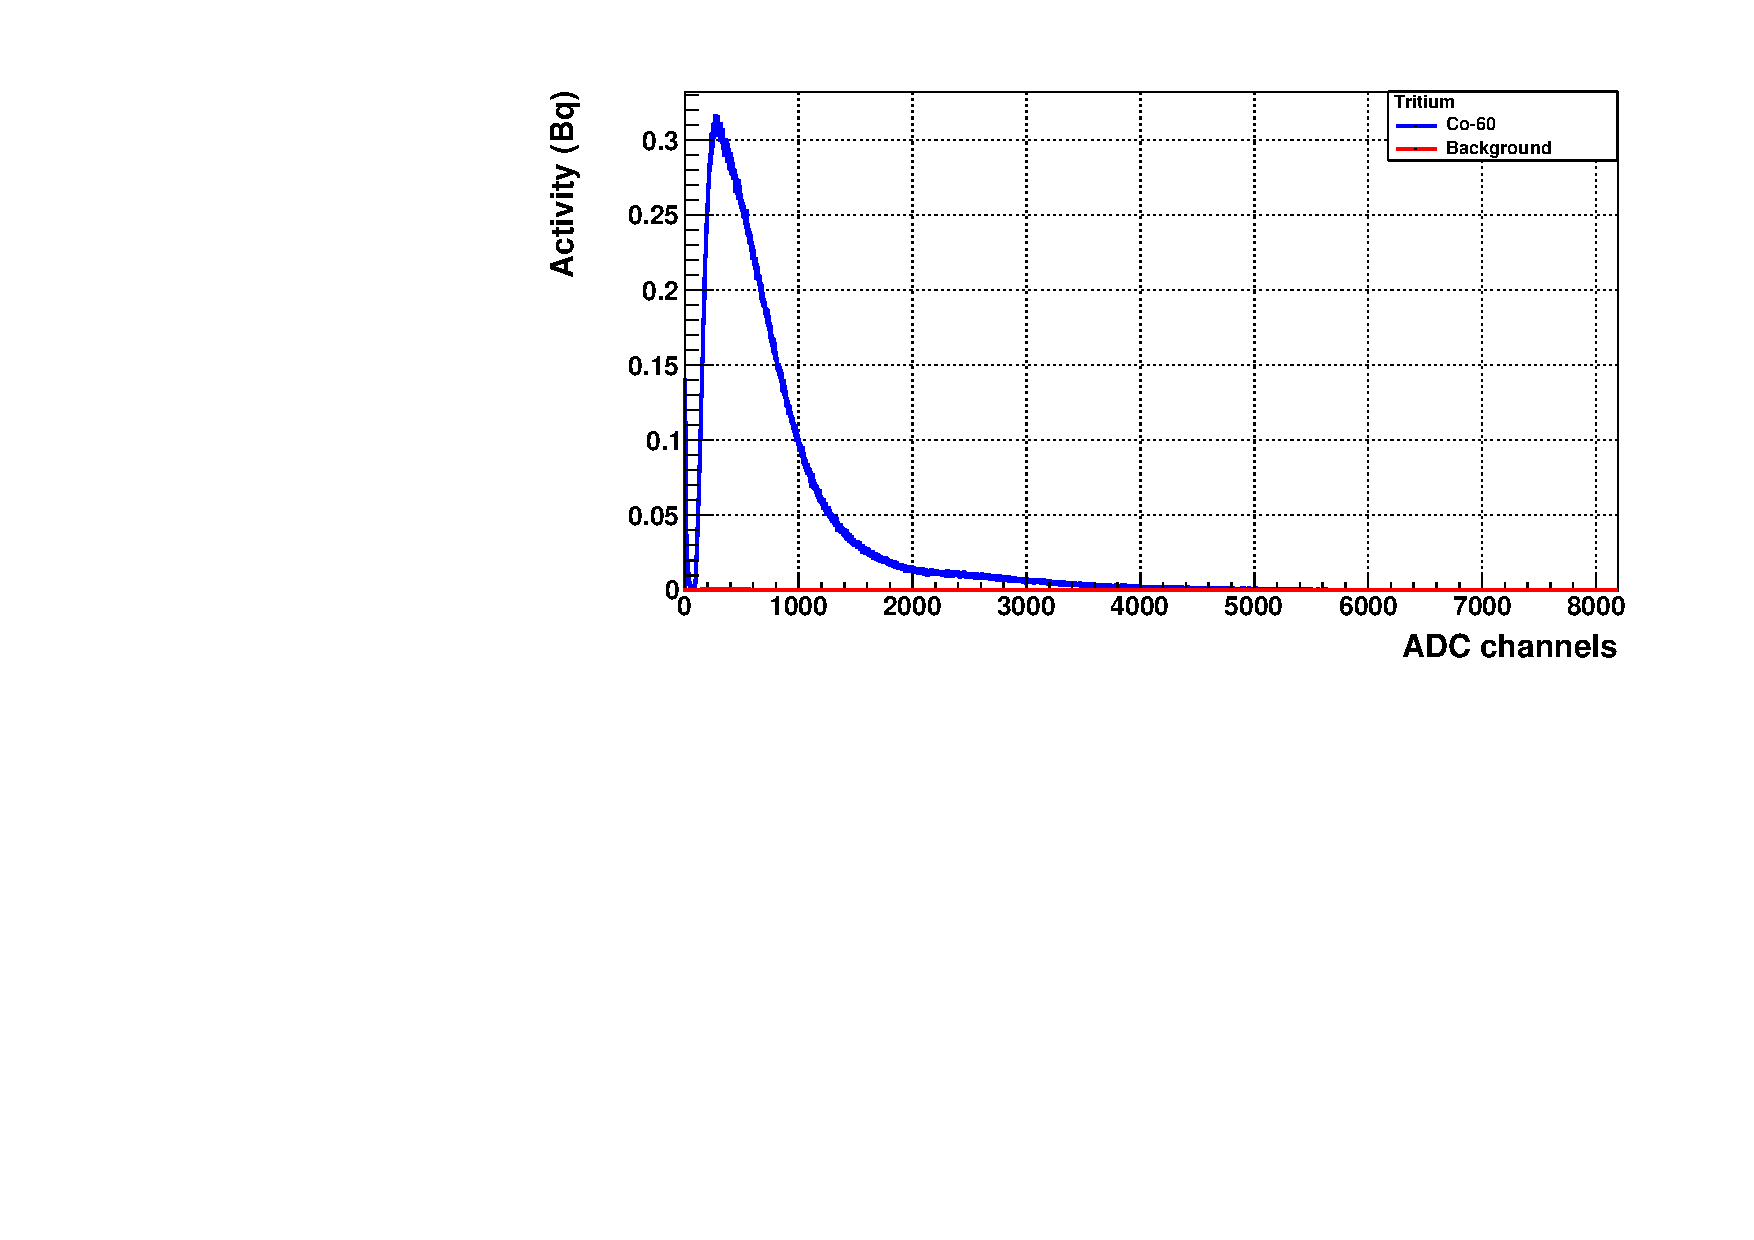
\includegraphics[scale=0.3]{LARAM/Polishing_effect/Second_try/No_polished/Co_60_no_polished.pdf}
\caption{Co-60 with fibers not polished}
\end{figure}

\column{0.5\textwidth}

\begin{figure}[hbtp]
\centering
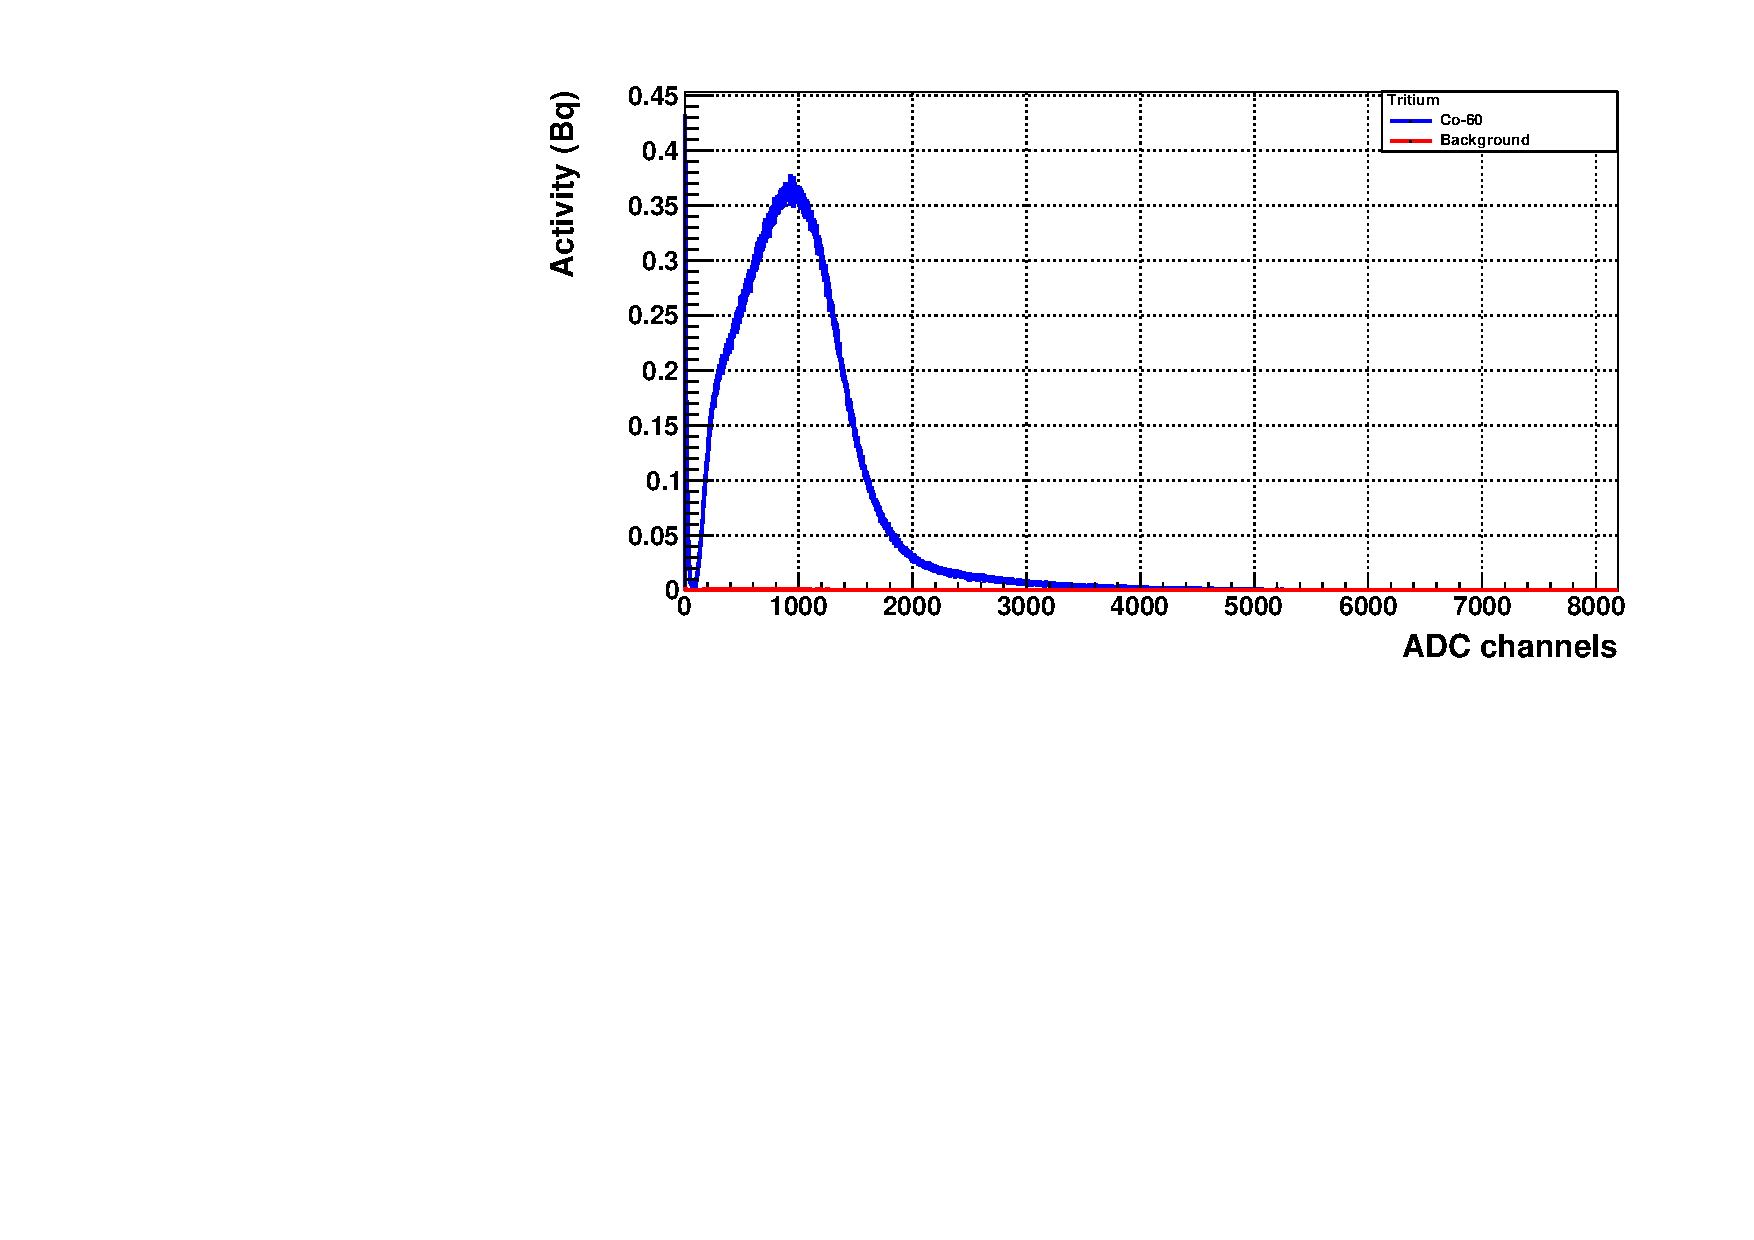
\includegraphics[scale=0.3]{LARAM/Polishing_effect/Second_try/Polished/Co_60_polished.pdf}
\caption{Co-60 with fibers polished}
\end{figure}

\end{columns}

\end{frame}

\begin{frame}
\frametitle{LARAM. Polishing effect with PMTs}
Second try

\begin{figure}[hbtp]
\centering
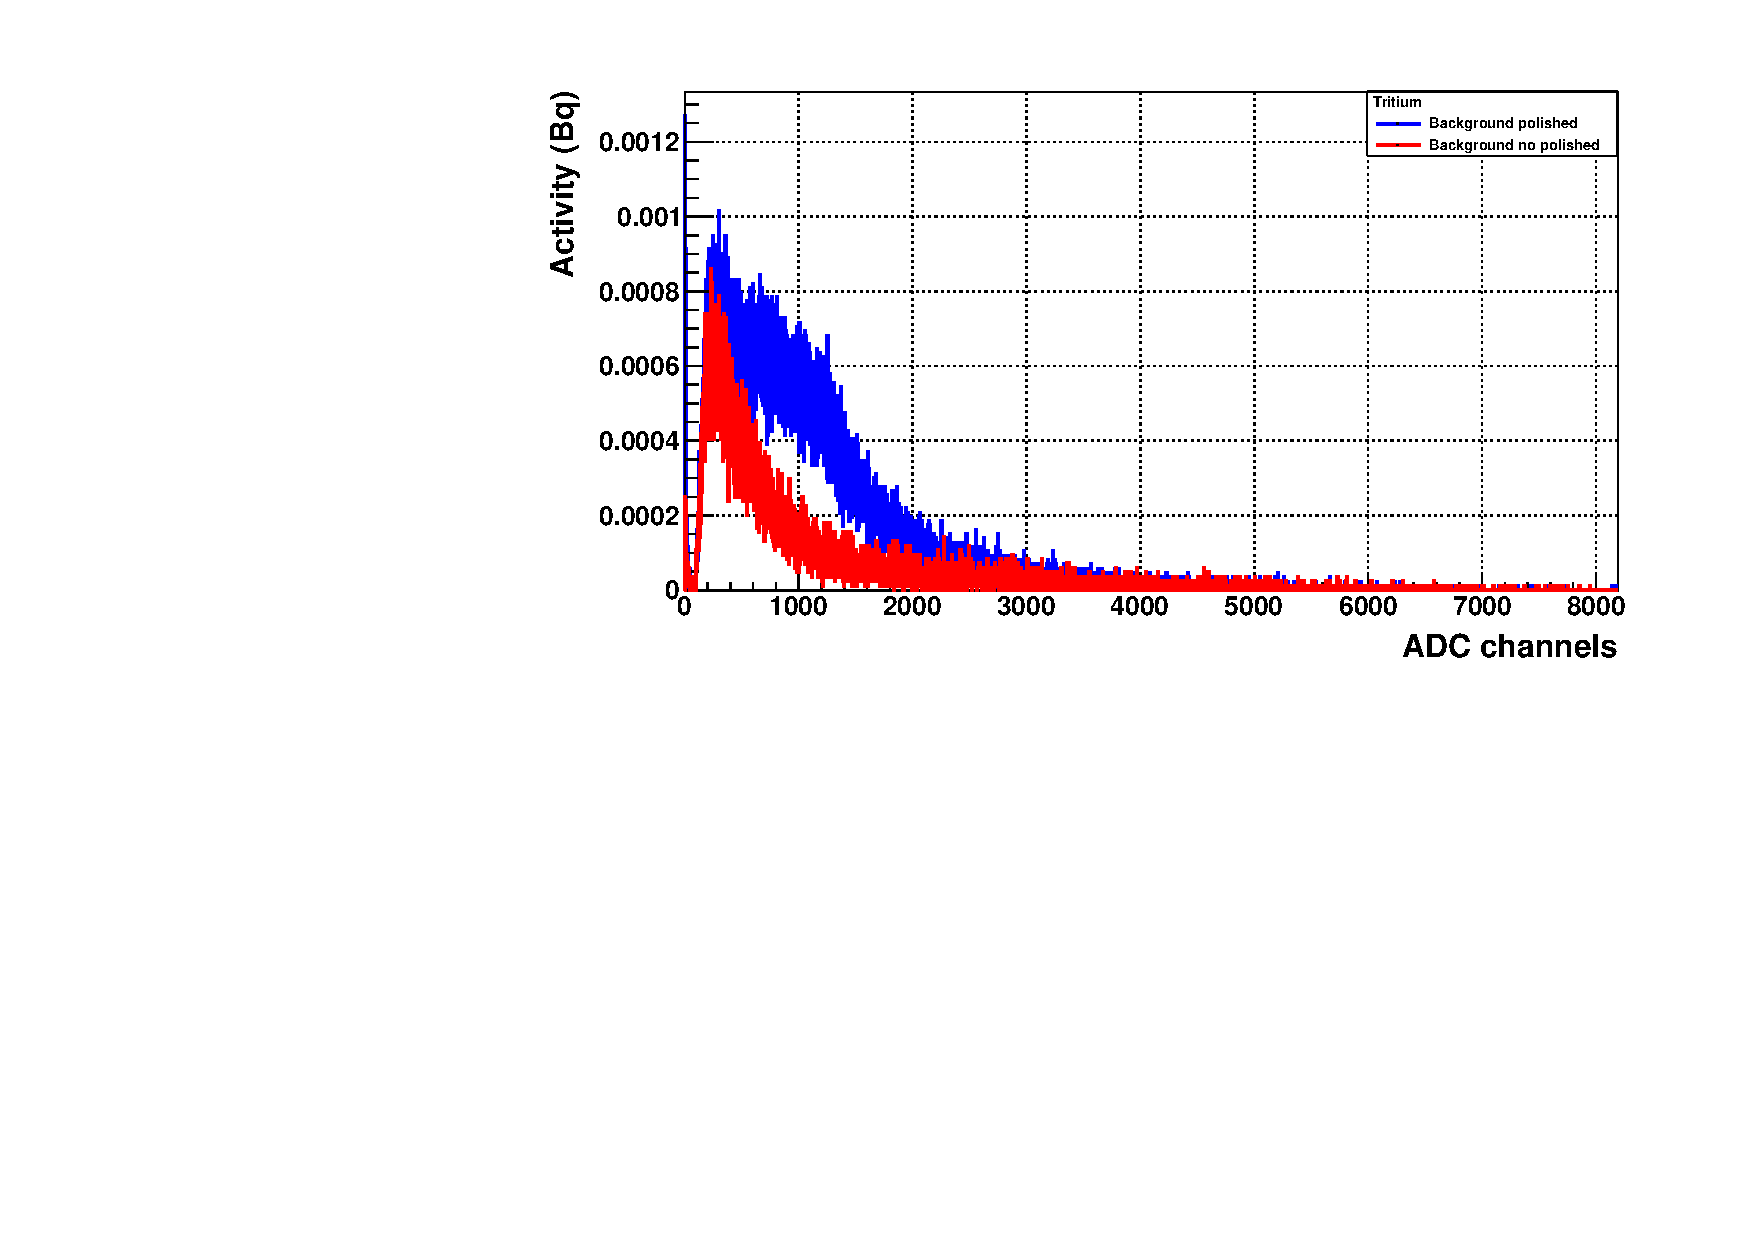
\includegraphics[scale=0.5]{LARAM/Polishing_effect/Second_try/Backgrounds.pdf}
\caption{Bunch with 25 fibers with 15 cm}
\end{figure}

\end{frame}

\begin{frame}
\frametitle{LARAM. Polishing effect with PMTs}
Second try

\begin{figure}[hbtp]
\centering
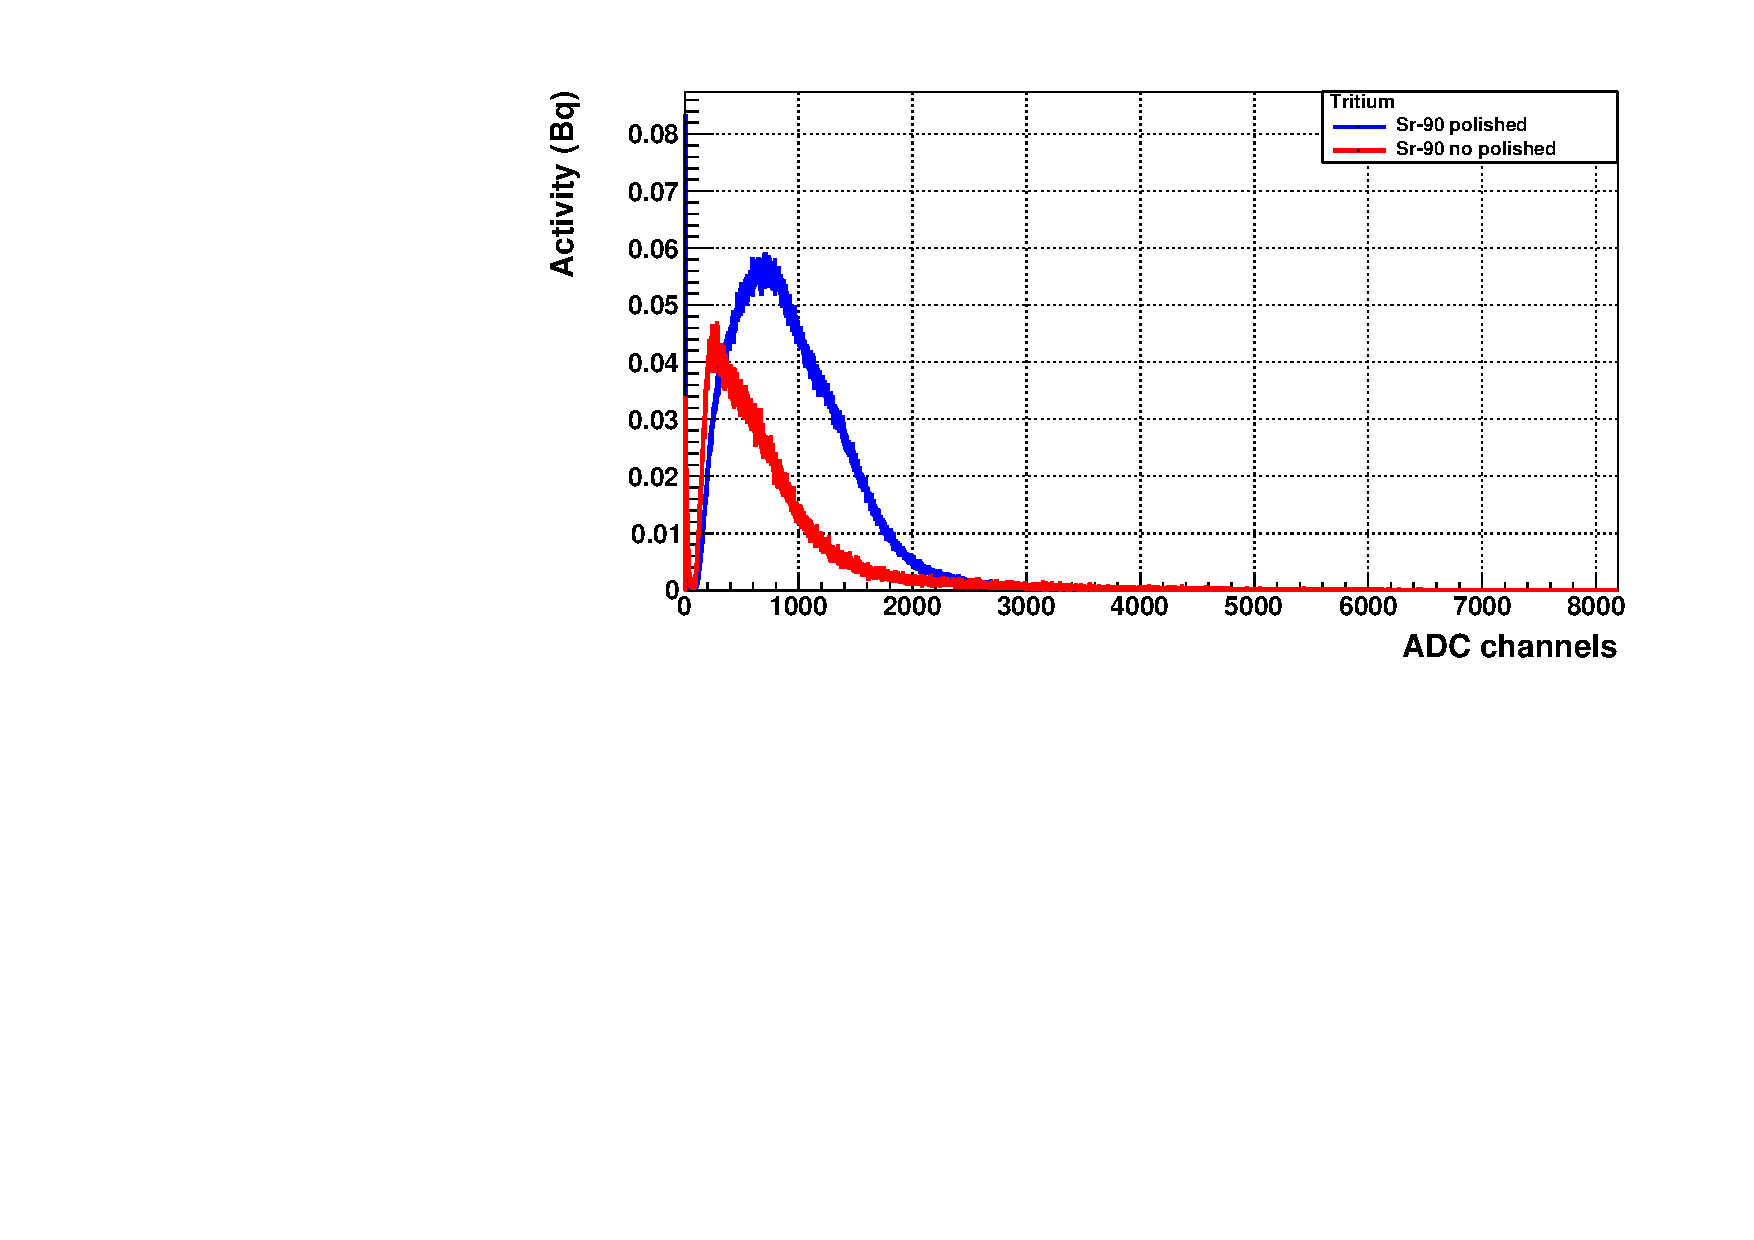
\includegraphics[scale=0.5]{LARAM/Polishing_effect/Second_try/Sr_90.pdf}
\caption{Bunch with 25 fibers with 15 cm}
\end{figure}

\end{frame}

\begin{frame}
\frametitle{LARAM. Polishing effect with PMTs}
Second try

\begin{figure}[hbtp]
\centering
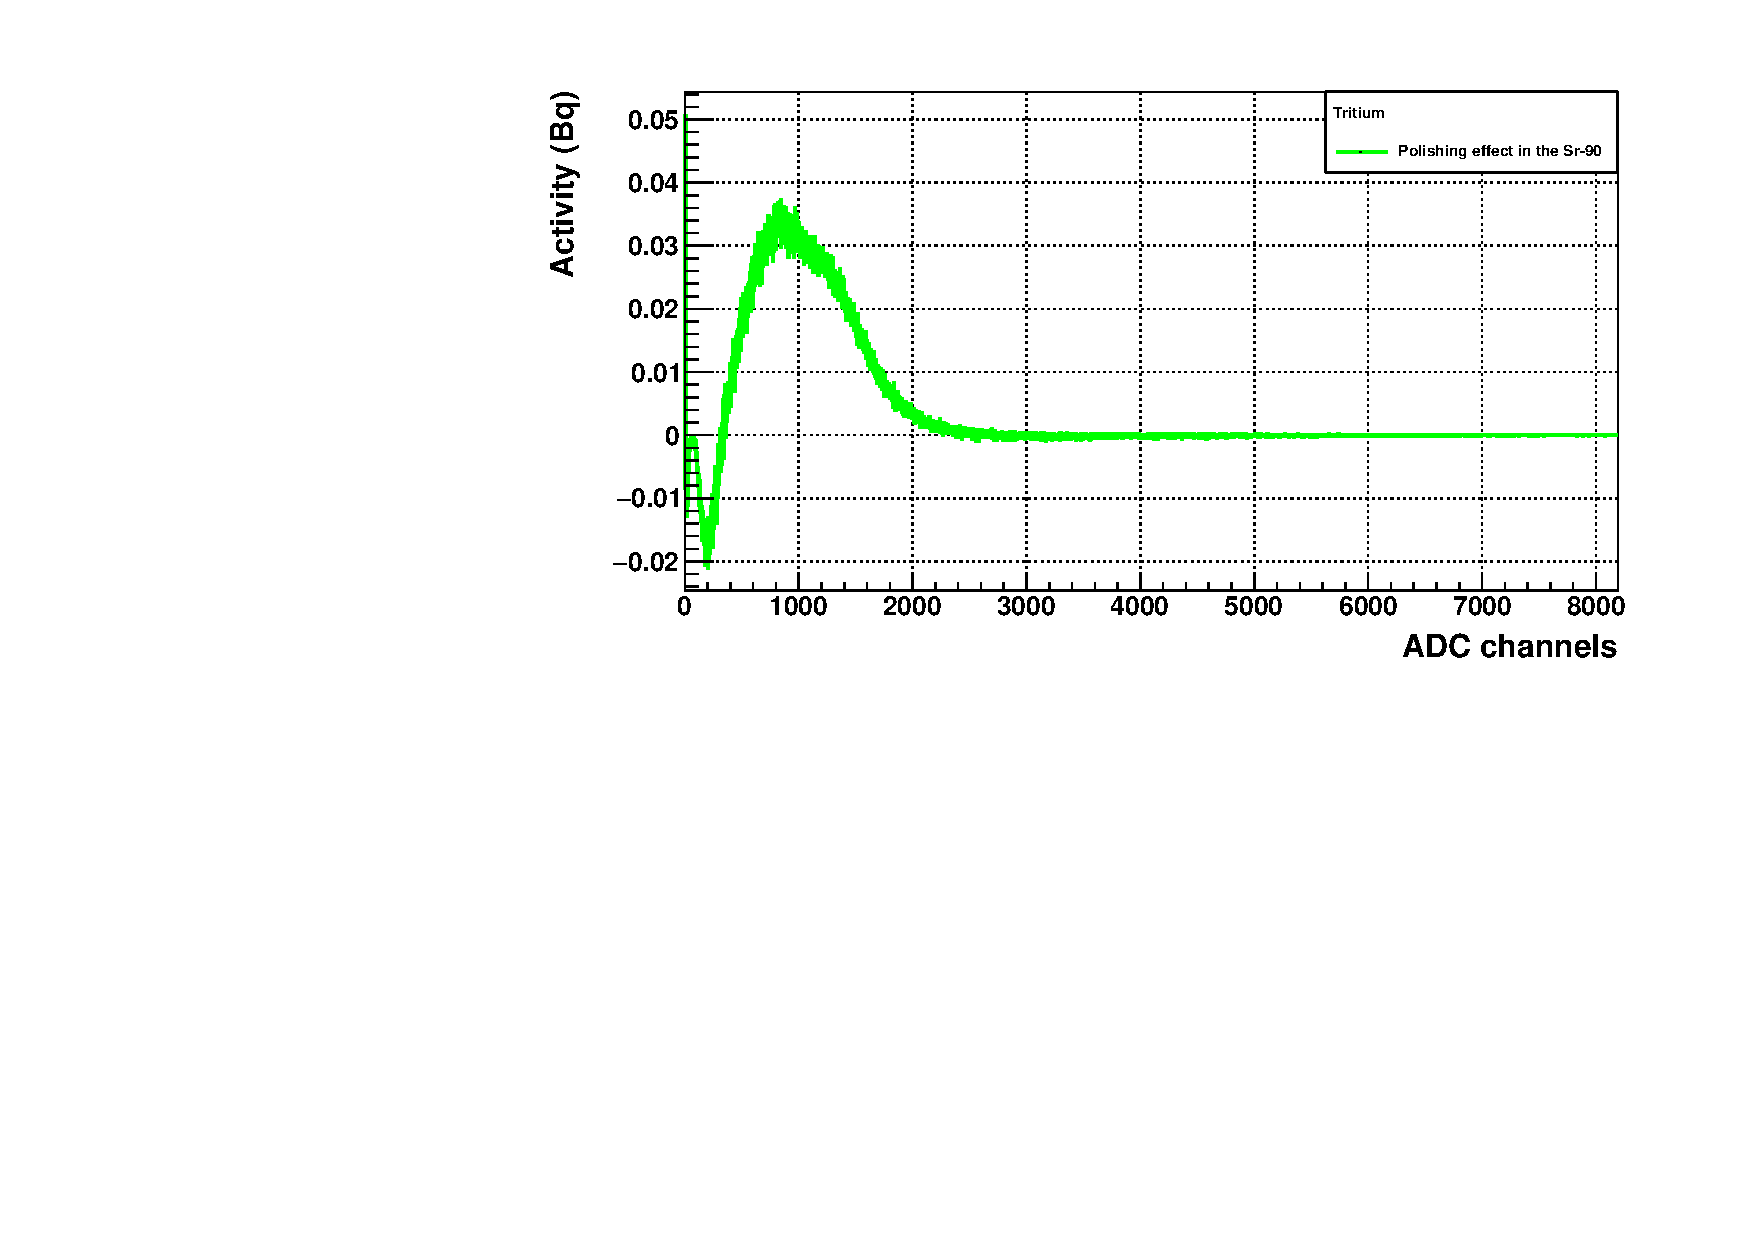
\includegraphics[scale=0.5]{LARAM/Polishing_effect/Second_try/Sr_90_clear.pdf}
\caption{Bunch with 25 fibers with 15 cm}
\end{figure}

\end{frame}

\begin{frame}
\frametitle{LARAM. Polishing effect with PMTs}
Second try

\begin{figure}[hbtp]
\centering
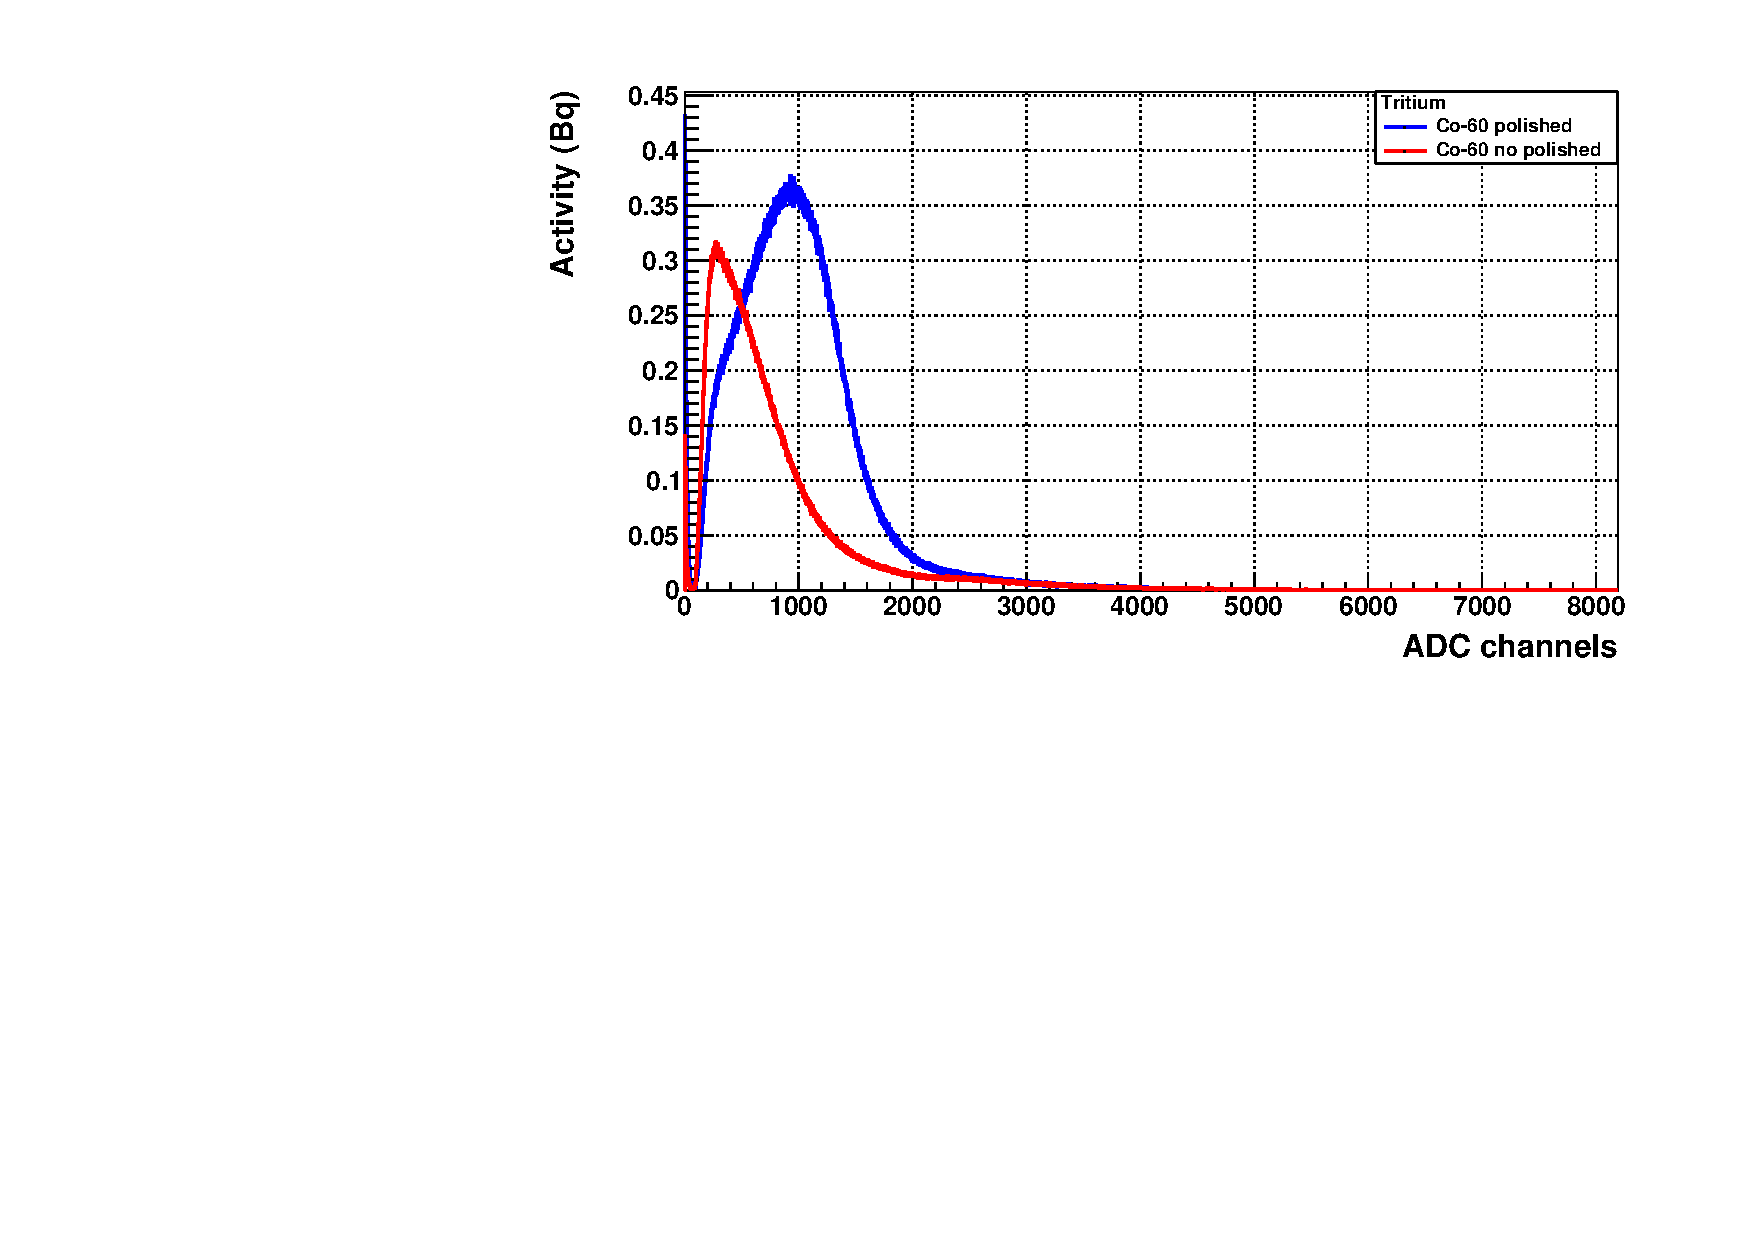
\includegraphics[scale=0.5]{LARAM/Polishing_effect/Second_try/Co_60.pdf}
\caption{Bunch with 25 fibers with 15 cm}
\end{figure}

\end{frame}

\begin{frame}
\frametitle{LARAM. Polishing effect with PMTs}
Second try

\begin{figure}[hbtp]
\centering
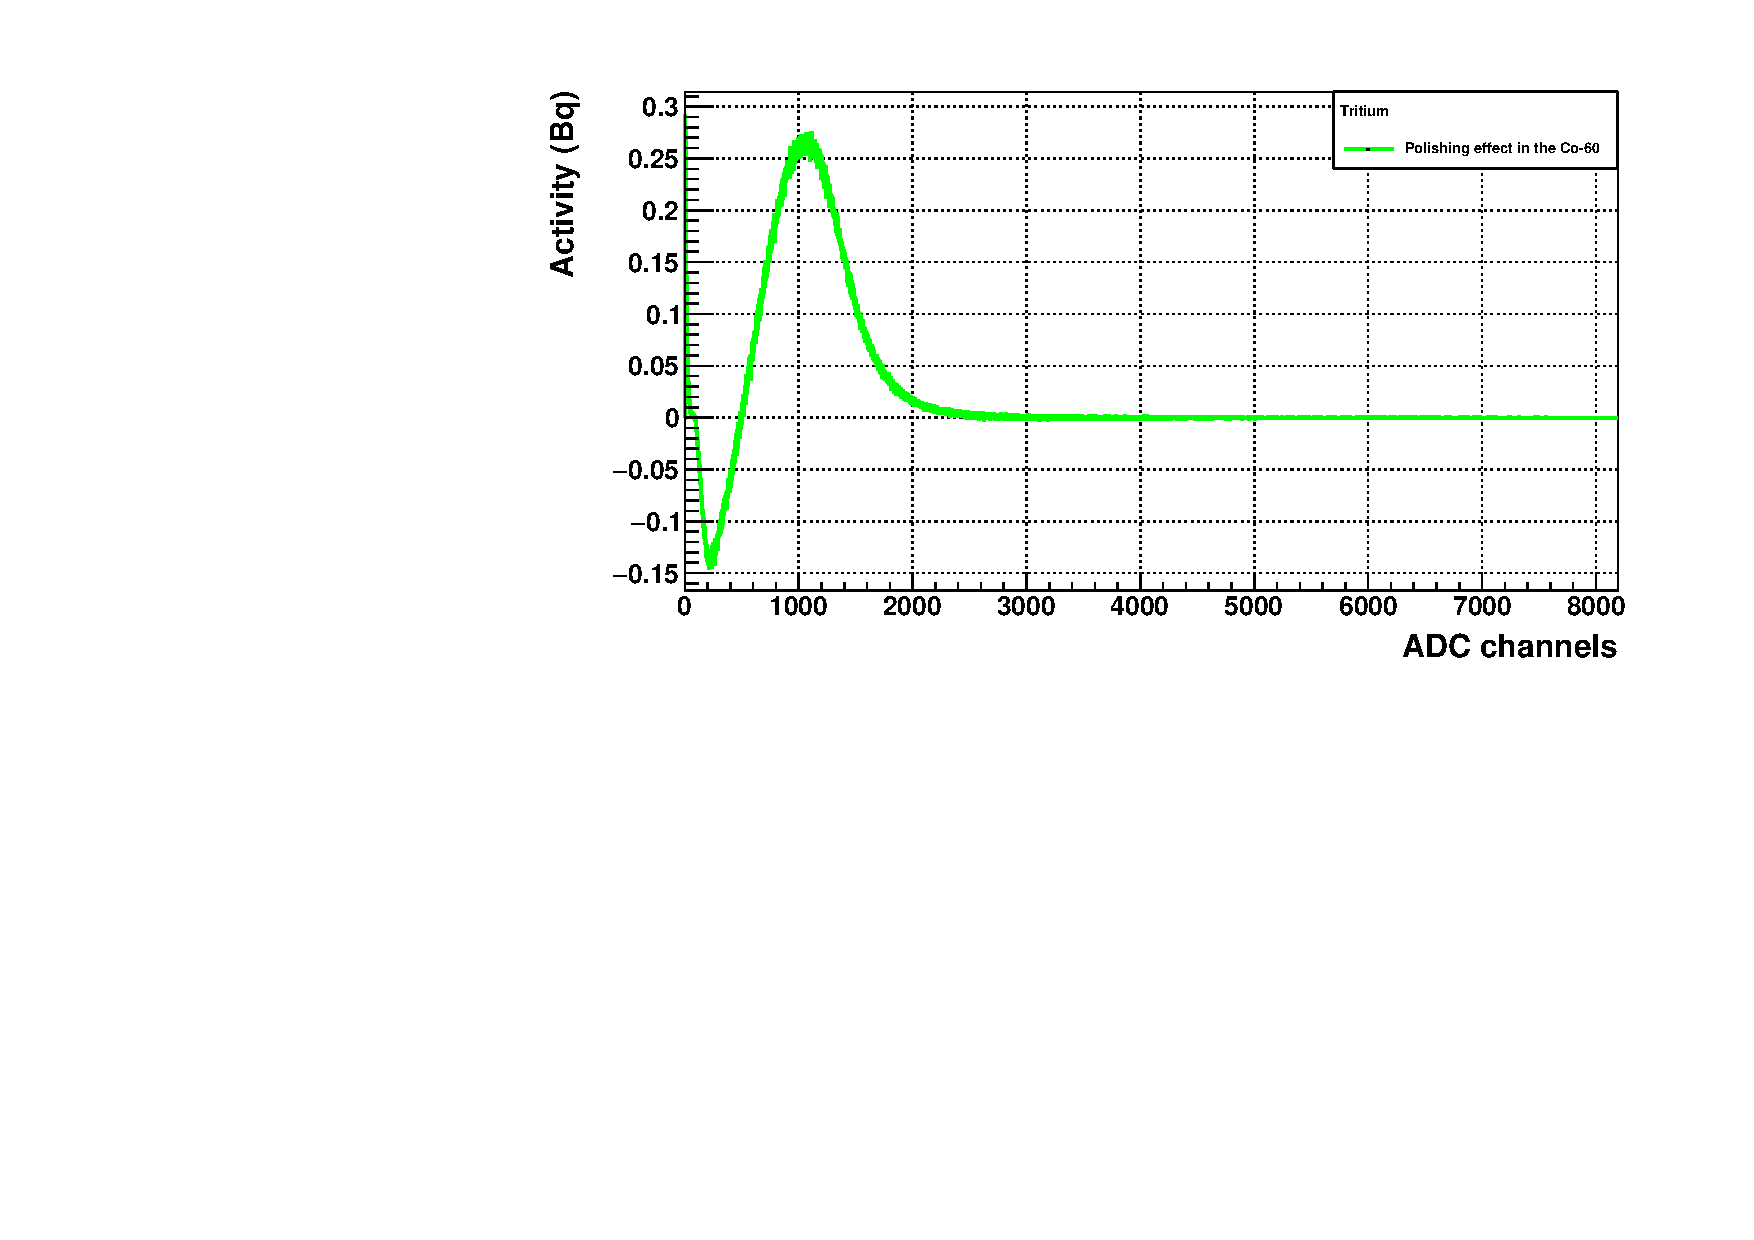
\includegraphics[scale=0.5]{LARAM/Polishing_effect/Second_try/Co_60_clear.pdf}
\caption{Bunch with 25 fibers with 15 cm}
\end{figure}

\end{frame}

\begin{frame}
\frametitle{LARAM. Polishing effect with PMTs}
Second try

\begin{table}
\begin{tabular}{l | c | c | c}
Source & Not polished & Polished \\
\hline \hline
Sr-90 & 33 & 64  \\ 
Co-60 & 243 & 424
\end{tabular}
\caption{Counts/second due to each source}
\end{table}

\end{frame}

\begin{frame}
\frametitle{LARAM. Future studies}

\begin{itemize}
\item{} I want to cuantify the effect of the clean process in the ICMOL room (Without ozone machine). I don't hope to obtain a better results but neither worse results.
\item{} I want to cuantify the damage due to the ozone machine (0, 30 seg, 1 min, 2 min, 5 min).
\item{} I want to obtain the measuring for several lengths of the fibers (5 cm, 10 cm, 15 cm and 20 cm). I can do it with this new setup.
\item{} other ideas?

\end{itemize}

\end{frame}

\begin{frame}
\frametitle{TRITIUM-IFIC 2. Coincidence effect}

MACRO

\end{frame}

\begin{frame}
\frametitle{TRITIUM-IFIC 2. Effect to the lead}

\begin{figure}[hbtp]
\centering
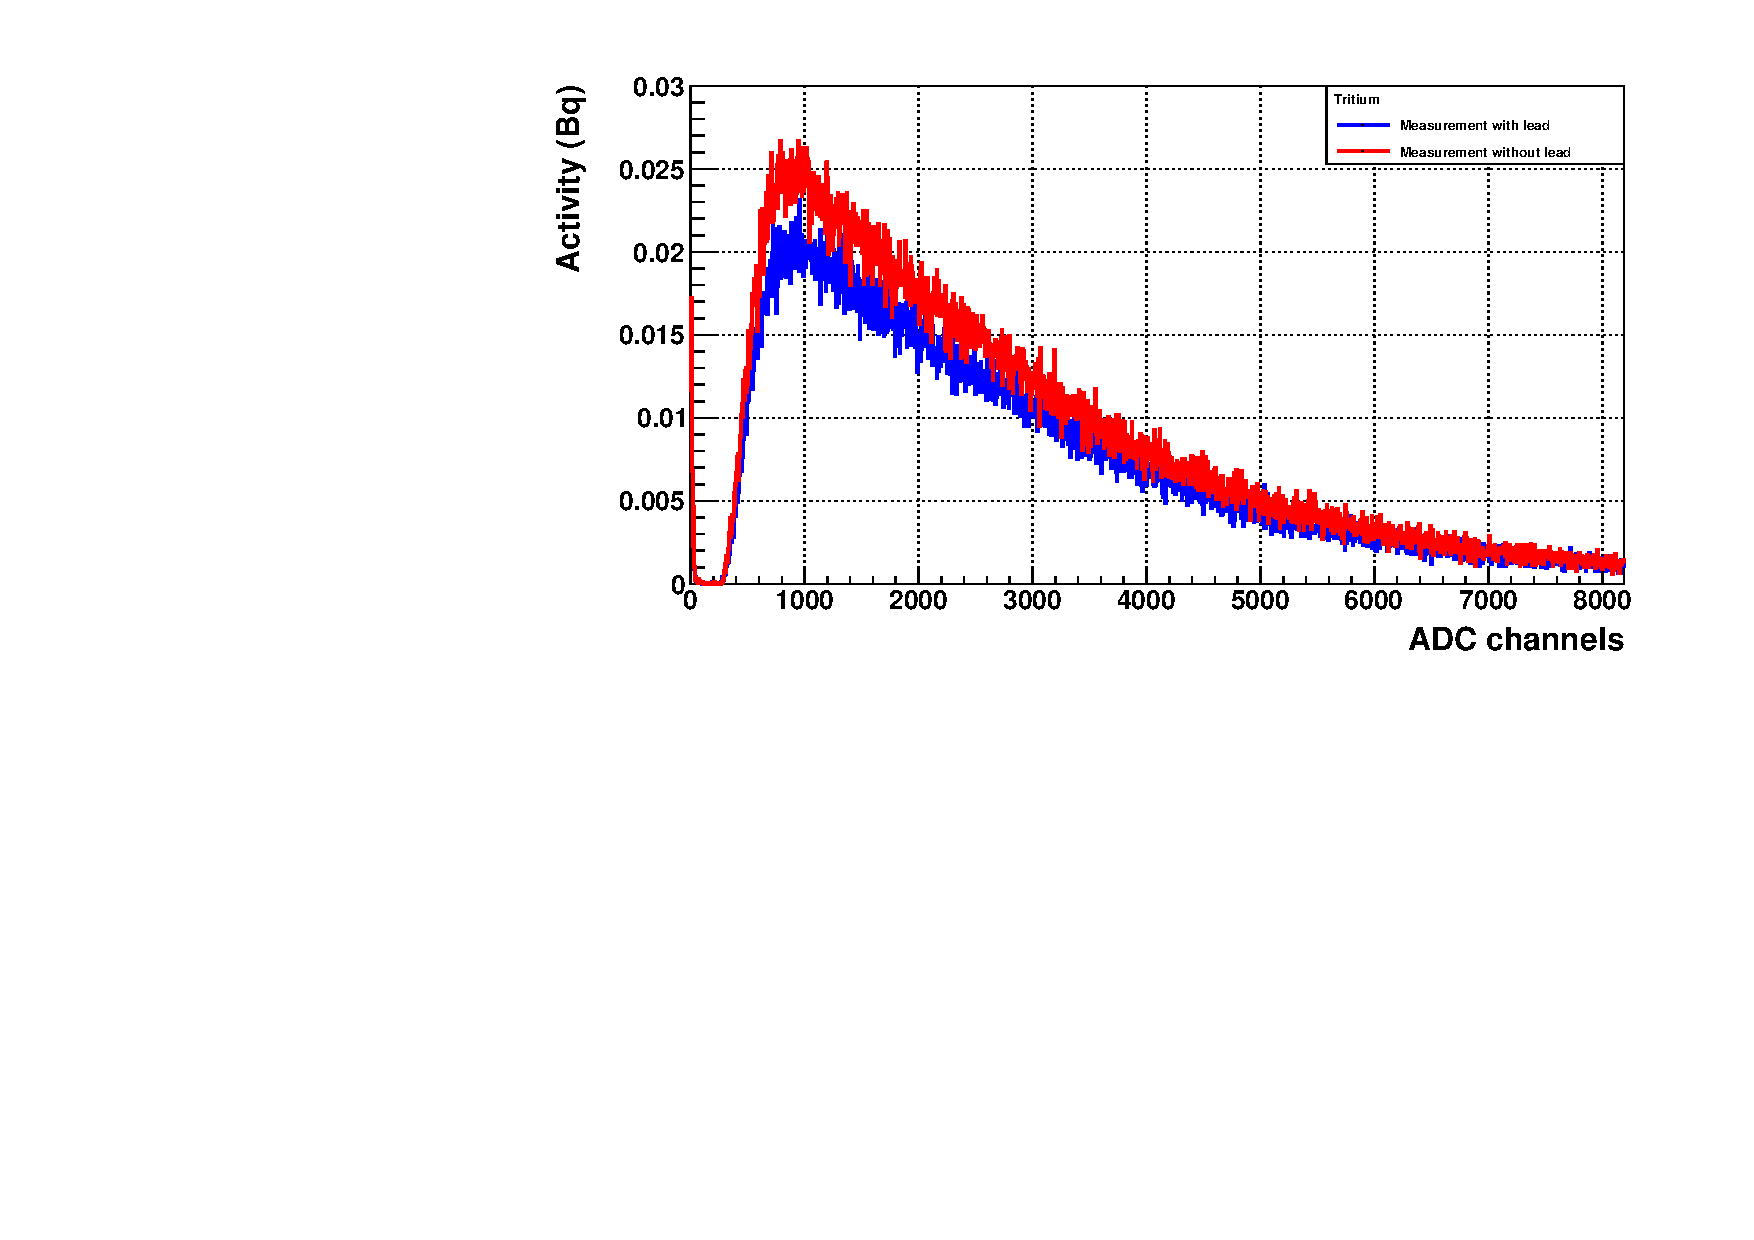
\includegraphics[scale=0.5]{TRITIUM2/With_without_lead.pdf}
\caption{Bunch with 25 fibers with 15 cm}
\end{figure}

\end{frame}

\begin{frame}
\frametitle{TRITIUM-IFIC 2. Effect to the lead}

\begin{figure}[hbtp]
\centering
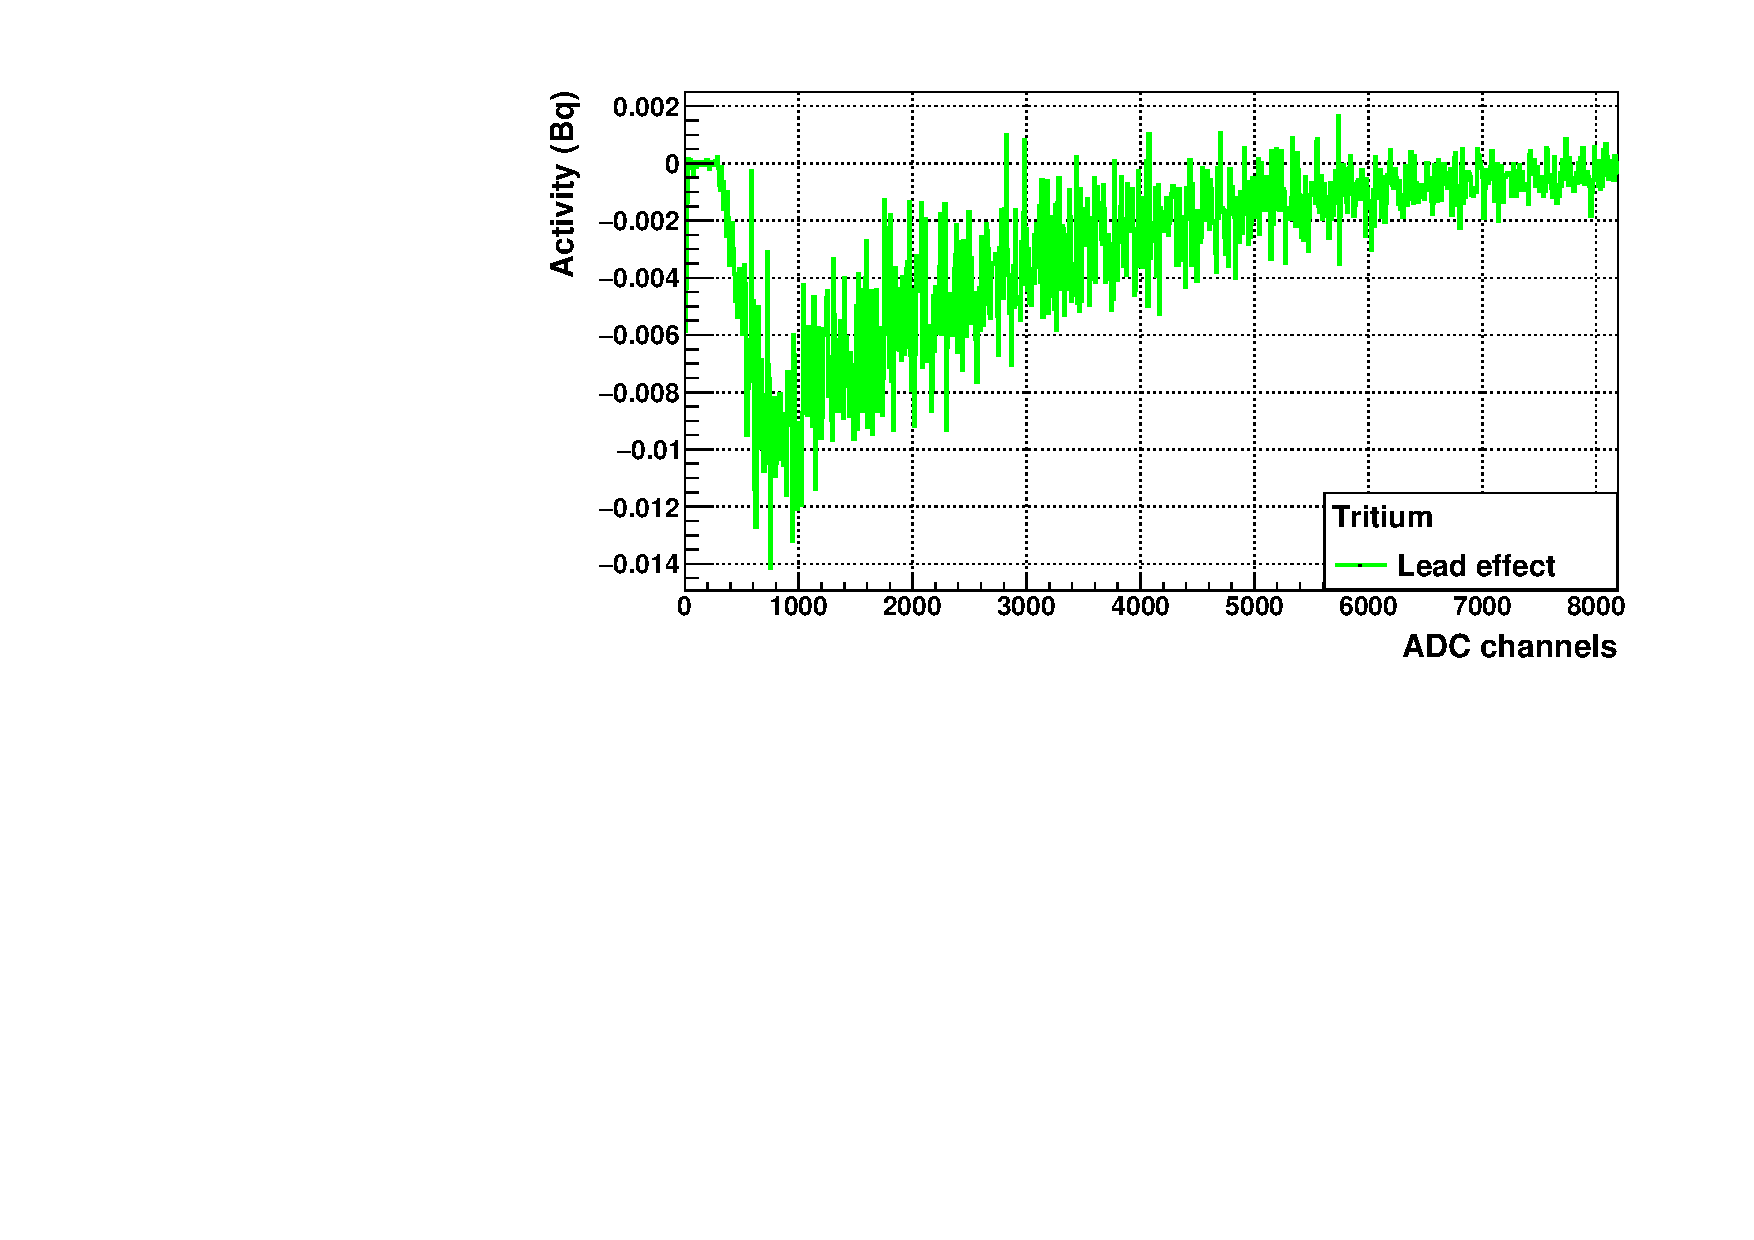
\includegraphics[scale=0.5]{TRITIUM2/Lead_effect.pdf}
\caption{Bunch with 25 fibers with 15 cm}
\end{figure}

\end{frame}

\begin{frame}
\frametitle{TRITIUM-IFIC 3.}

\begin{itemize}
\item{} I have managed the purchase of teflon, PMMA windows, belts and I/O water.
\item{} The teflon have already arrived. The mechanism has started with the construction of this prototype. He is close to finish.
\item{} I bought I/O water pieces from TEBYC company.
\item{} I bought belts from TECNIMAN company.
\item{} I have the PMMA windows from Hermanos Monge company (free).
\item{} The best idea is build two detectors (one for the background and other for the tritium signal).
\item{} I have 600 fibers polished. I will polish 600 fibers more.
\item{} I have to obtain the transmision spectrum for this new windows.
\end{itemize}

\end{frame}


\end{document}



